\documentclass[twoside]{report}

% the following conforms with UoN's guidelines on Thesis formats
%  I'm not sure about the 1.5 line spaceing: looks a bit to much
\usepackage[a4paper,width=150mm,top=30mm,bottom=20mm]{geometry}
%\linespread{1.25} % this is equivalent to 1.5 line spacing in MS Word

\usepackage[T1]{fontenc}
\usepackage[utf8]{inputenc}
\usepackage[australian]{babel}

\usepackage{csquotes}

\usepackage[hidelinks]{hyperref}

%\usepackage{showlabels}

\usepackage{parskip}

\usepackage{microtype}

\usepackage[backend=biber]{biblatex}
\addbibresource{references.bib}

\usepackage{amsthm,amsfonts,amssymb,amsmath,mathtools,graphicx}

\usepackage[linesnumbered,ruled]{algorithm2e}

% defines a function type
\SetKwProg{Fn}{Function}{}{end}

% the following are algorithms that will be defined
%  in pseudocode within this document
\SetKwFunction{WP}{WordProblem}
\SetKwFunction{COMP}{compare}

\SetKwFunction{SORT}{sort}
\SetKwFunction{MERGE}{merge}
\SetKwFunction{MERGEFINAL}{mergeFinal}

% ensures that the pseudocode doesn't use italics 
\SetArgSty{textup}

\usepackage{subcaption}

\usepackage[capitalise,noabbrev]{cleveref}

\usepackage{tikz}

\usepackage{siunitx}

\usepackage{styles/doubleangle}
\usepackage{styles/theoremstyles}
\usepackage{styles/comments}
\usepackage{styles/notation}

\title{
	{\LARGE Geodesic Growth of the Fabrykowski-Gupta Group}\\
	{\Large Honours Thesis}\\
	{\large University of Newcastle}\\\ \\
	{
		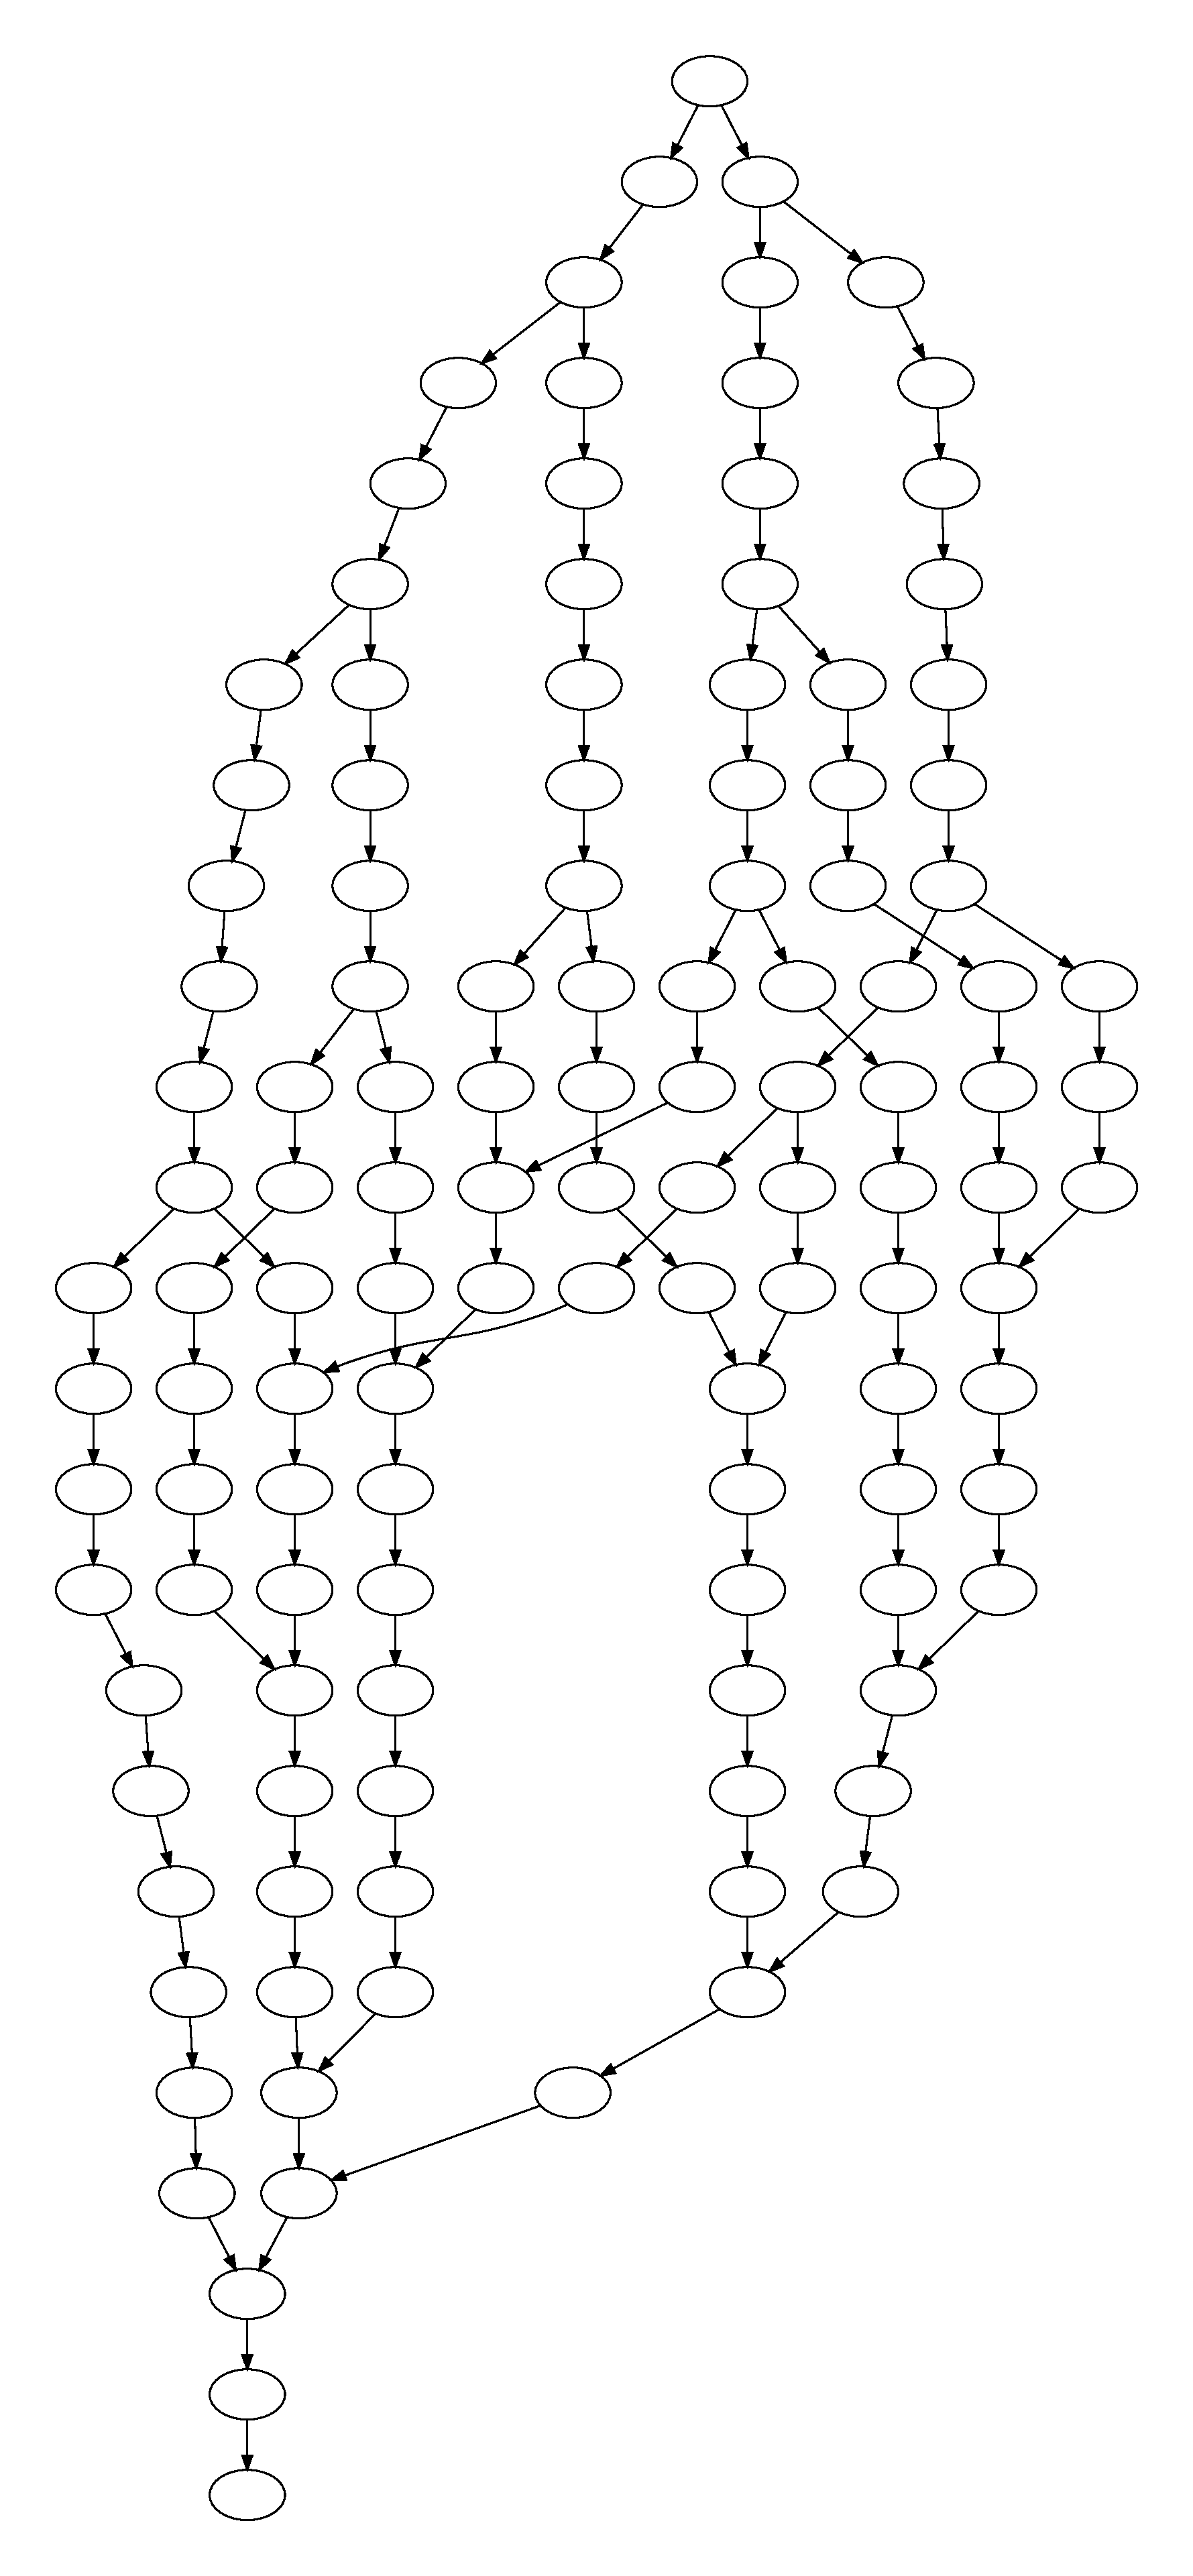
\includegraphics[height=10cm]{figures/cover}
	}
}
\author{
	Author:\\Alex Bishop
\and
	Supervisor:\\A/Prof Murray Elder
}
\date{Submitted: 27 October 2017}

\hypersetup{pdfinfo={
	Author={Alex Bishop},
	Title={Geodesic Growth of the Fabrykowski-Gupta Group},
	Subject={Geometric Group Theory},
	Keywords={Fabrykowski-Gupta;Group Theory;Geodesic Growth;Complexity Analysis},
}}

%\includeonly{chapters/results}

\begin{document}

\pagenumbering{gobble}
\maketitle

\clearpage
\pagenumbering{roman}

\chapter*{Abstract}

An open question in geometric group theory is whether there exists a group with intermediate geodesic growth.
That is, a group for which the function which counts the number of length $n$ geodesics grows faster than any polynomial and slower than any exponential; a potential example for this property is the Fabrykowski-Gupta group.

This thesis will present an efficient algorithm for computing the geodesics of the Fabrykowski-Gupta group with the objective being to provide a computation-based experimental method for studying the geodesic growth of this and similar examples.
This algorithm will be shown to have a worst-case time complexity given by
\[
  O\left(
    \sum_{\ell=1}^{n} s(\ell-1) \log s(\ell-1) \ell \log \ell 
  \right)
\]
where $n$ is the length of geodesic to generate, and $s(n)$ is the strict growth of the Fabrykowski-Gupta group, which will be shown to be a great improvement over the previously known brute force method.
This paper will end with a presentation of the data generated by the algorithm.

\chapter*{Statement of Authenticity}

I hereby certify that the work embodied in the thesis is my own work, conducted under normal supervision.

The thesis contains no material which has been accepted, or is being examined, for the award of any other
degree or diploma in any university or other tertiary institution and, to the best of my knowledge and
belief, contains no material previously published or written by another person, except where due reference
has been made in the text. I give consent to the final version of my thesis being made available worldwide
when deposited in the University's Digital Repository, subject to the provisions of the Copyright Act 1968
and any approved embargo.

\vspace*{1cm}

\begin{center}
\footnotesize
\begin{tabular}{l l l}
	\makebox[0.3\linewidth]{\hrulefill}&\makebox[0.3\linewidth]{\hrulefill}&\makebox[0.3\linewidth]{\hrulefill}\\
		NAME                           & SIGNATURE                         & DATE (DD/MM/YYYY)
\end{tabular}
\end{center}


\chapter*{Acknowledgements}

First and foremost, I would like to thank Murray Elder for being my supervisor through honours even after changing universities, for sending me to the AMSI summer school so that I could learn about geometric group theory, and for making it possible for me to attend three international conferences in Spain related to my research (something that would otherwise be unheard-of for an Honours student).
I would also like to thank Murray Elder for his help in filling out the terse forms that universities require and for his suggestions for my thesis.

I would like to thank Thomas Murray for his work on a summer research project which has become a preliminary study into the plausibility of this honours thesis.

I thank Anne Thomas and Lawrence Reeves for teaching me geometric group theory, without whom I wouldn't have an understanding of the area and would thus be lost with my project.
Also, I thank the organisers of the 2017 AMSI summer school for running this course.

I thank the organisers of the 2017 conferences yGAGTA and GAGTA, and the organisers of the 2017 conference Groups of Intermediate Growth in Seville.


\tableofcontents

\clearpage
\pagenumbering{arabic}

\chapter{Introduction}

Introduced, independently, in 1955 by A. S. \v{S}varc  %Albert Schwarz 
\cite{SvarcEquivClass} and in 1968 by John Milnor \cite{MilnorEquivClass}, the concept of \emph{growth} has been at the centre of many profound results in group theory.
The concept will be formally introduced and defined in \cref{sec:growth-functions,sec:interGrowth} of the next chapter.
Informally, a growth function counts the number of distinct group elements which may be represented as a composition of $n$, or fewer, generators; such functions are usually viewed with respect to their asymptotic behaviours as described by \v{S}varc and Milnor in their respective papers as aforementioned.

In 1968, it became apparent that every known class of group in the literature possessed a growth function that was either polynomial $n^d$ with $d$ a non-negative integer, or exponential $e^n$.
Thus, Milnor formally posed the question as to whether these were the only possible growth types i.e.\ whether there exists a group whose growth type is neither polynomial of a non-negative integer degree nor exponential \cite{Milnor1968}.
This question was partially answered in 1972 when Hyman Bass showed that if a group has growth of polynomial type $n^\alpha$, then $\alpha$ is a non-negative integer \cite{PolynomialDegree}.
The remaining question of the existence of intermediate growth (i.e.\ growth that is faster than any polynomial and slower than an exponential) remained unsolved until 1984 when Rostislav Grigorchuk proved a particular group, which he first introduced in \cite{GrigFirst}, to have such a growth type \cite{GrigInterm}; for a proof of the intermediate growth of this group and an introduction to intermediate growth, the reader is directed to the survey article \cite{GrigPak}.

Grigorchuk's example  has been the focus of much of the research into intermediate growth.
Many of the known classes of groups with intermediate growth are extensions of Grigorchuk's original example or one of its generalisations, as introduced in \cite{GrigInterm}.
In fact, using this generalisation, Laurent Bartholdi and Anna Erschler were able to show the existence of a continuum of potential intermediate growths of groups \cite{PossibleIntermGrowth}; in particular, they showed that if $\eta$ is the positive root of the polynomial $x^3 - x^2 -2x - 4$, then given any function $f : \mathbb{R}_+ \to \mathbb{R}_+$ such that $f(2R) \leq f(R)^2 \leq f(\eta R)$ for all sufficiently large $R$, then there exists a group with growth equivalent to $f$;
further, such a group is equivalent to a wreath product of a generalised version of Grigorchuk's construction by a finite group.

As mentioned before, there are deep connections between properties of groups and their growth, one such example being the famous theorem of Mikhael Gromov, that is, that a group has polynomial growth if and only if it is virtually nilpotent \cite{GromovTheorem}.
Furthermore, there are still many open problems remaining in the study of growth, one such open problem, introduced in \cite{GrigGap}, is whether there exists a group with intermediate growth that is equivalent to or slower than $e^{\sqrt{n}}$.

This thesis is interested in a similar concept to growth known as \emph{geodesic growth}; informally, a geodesic growth function counts the number of geodesics, with respect to some chosen generating set, that may be constructed from the composition of $n$, or fewer, generators.
Similar to growth functions, geodesic growth functions can be studied with respect to their asymptotic properties.
Such asymptotic properties of geodesic growth are of interest within this thesis.

Unlike the usual concept of growth, at present, geodesic growth has received little attention in the literature.
Attempts have been made to generalise theorems, such as Gromov's, to geodesics. In \cite{OnGroupsPolynomial} it was shown that if a group $G$ contains an element $x \in G$ whose normal closure is an abelian subgroup of finite index, then there is a generating set with respect to which the geodesic growth of $G$ is polynomial.
Although this paper didn't present a classification of groups with polynomial geodesic growth, it did show the existence of non-obvious groups (i.e.\ groups other than $\mathbb{Z} = \left\langle z \, \middle\vert - \right\rangle$ with respect to its usual generating set) with polynomial geodesic growth.

This thesis is interested in the open question, similar to Milnor's in 1968, whether there exists a group with a generating set with respect to which the geodesic growth is intermediate.

A natural starting point in the search for a group with intermediate geodesic growth would be Grigorchuk's first construction (of a group with intermediate growth) \cite{GrigFirst}.
However, it was shown in an unpublished paper by Murray Elder, Mauricio Gutierrez, and Zoran \v{S}uni\'c, a result that was later released as part of the PhD thesis of Julie Br\"onnimann \cite{Julie2016GeodesicGrowth}, that the geodesic growth of this group is exponential; this proof was accomplished by considering the geodesics which appear in the $n$-th level Schreier graphs of the group.
Further, using this technique Br\"onnimann was able to show that almost all groups acting on regular rooted trees (which she was aware of in the literature) to be of exponential geodesic growth when considered with respect to their usual generating sets, the only exception being the so-called \emph{Fabrykowski-Gupta group}.

The Fabrykowski-Gupta group was first defined by Jacek Fabrykowski and Narain Gupta in \cite{FabGuptaI}.
This paper also showed the group to have intermediate growth, however, a problem in this proof led to a second paper \cite{FabGuptaII} by Fabrykowski and Gupta, followed by a third proof in \cite{OnGrowth} by Bartholdi and Floriane Pochon which provided some missing details of \cite{FabGuptaII}.
This result is of interest in this thesis as the geodesic growth of a group is bounded from below by its usual growth, thus for a group to have intermediate geodesic growth, it can have regular growth which is intermediate at most.

The Fabrykowski-Gupta group remains a potential example of intermediate geodesic growth, and thus this group is the study of this thesis.
This paper will present a computation-based technique for studying the geodesic growth of Fabrykowski-Gupta, and similar, groups.

In the literature, few groups have known geodesic growth types beyond the classification of either polynomial % of geodesic.
or exponential.
For such groups, their geodesic growth types are known explicitly.
Examples of such groups are abelian groups \cite{Julie2016GeodesicGrowth}, and classes of right-angled Artin groups and Coxeter groups \cite{GeodesicsCoxeterI,GeodesicsCoxeterII}.
Hence, few general techniques of studying geodesic growth are known.

Given the lack of techniques available in the literature, this thesis will present an efficient algorithm for generating the geodesics of the Fabrykowski-Gupta group (see \cref{chp:FG-group,chp:generating-geodesics} for this algorithm and its time complexity), and collecting them into their respective equivalence classes as it does so.
The idea of using this algorithm is to generate a sufficient amount of data such as to find patterns therein, and thus to assist in constructing theorems about the geodesic growth of this group.

It will be shown that this geodesic generating algorithm is an improvement, with respect to time complexity, over the previously known brute force method.
Further, remarks will be made as to the possibility of extending this algorithm to similar groups.
This thesis will conclude with a summary of the results which were obtained from running this geodesic generating algorithm.


\chapter{Preliminaries}

This chapter will introduce the reader to the notation and definitions that will be used throughout this thesis.
This chapter is not intended to be an introduction to group theory.
It is assumed that the reader is familiar with the basics of geometric group theory, such as, presentations and Cayley graphs.
For an introduction to the basics of geometric group theory, the reader is directed to the lecture notes \cite{AMSInotes,neumann1996short} and the book \cite{clay2017office}.

\section{Basic Notation}

Within this chapter and throughout this thesis, unless otherwise stated, $G$ will denote an arbitrary group with finite generating set $X$.

\begin{definition}
	Let $x,a\in G$, then the \emph{conjugate} of $x$ by $a$, denoted $x^a$, is defined as \[ x^a = a^{-1} x a \]
\end{definition}

\begin{definition}
	Let $x,y \in G$, then \emph{commutator} of $x$ and $y$, denoted $[x,y]$, is defined as \[ [x,y] = x^{-1}y^{-1}xy \]
\end{definition}

\begin{definition}
	All group actions are \emph{left group actions}.
	For example, let $G$ act on some given set $X$, and let $g,h\in G$ and $x \in X$, then
	\[
	  ( g h ) \cdot x = g \cdot ( h \cdot x)
	\]
	That is, the right-most action, $h$, is applied first.
\end{definition}

\begin{definition}
	The \emph{free group} on a set $X$, denoted $\F(X)$, is the group generated by freely reduced words in $\left( X \cup X^{-1} \right)^\ast$, where composition is concatenation followed by free reduction.
\end{definition}

\begin{definition}
	For the purpose of this thesis the set of \emph{natural numbers}, $\mathbb{N}$, will include zero.
	\[
	  \mathbb{N}
	  =
	  \left\lbrace
	    0, 1, 2, \ldots
	  \right\rbrace
	\]
	If zero is to be excluded, then the notation $\mathbb{N}_+$ will instead be used.
\end{definition}

\begin{definition}
	A function $f : \mathbb{N} \to \mathbb{R}$ is said to be \emph{submultiplicative} if \[ f(n + m) \leq f(n) \cdot f(m) \] for each $n,m \in \mathbb{N}$.
\end{definition}

\begin{example}
	Every polynomial, $x^\alpha$ with $\alpha \geq 0$, and exponential, $\alpha^x$ with $\alpha > 1$, is submultiplicative when considered as functions that map $\mathbb{N} \to \mathbb{R}_{\geq 0}$.
\end{example}

\begin{definition}
	$\Cay(G,X)$ shall denote the \emph{Cayley graph} of $G$ with respect to a generating set $X$.
\end{definition}

\newpage
\section{Words, Lengths and Geodesics}

For any group $G$ with generating set $X$, it is possible to define a length on the elements of $G$ based on representations by words in the language $\left( X \cup X^{-1} \right)^\ast$.
This definition of length becomes important when defining the growth functions of the following section.

\begin{definition}
	\label{def:word-length}
	Let $w = w_1 w_2 \cdots w_n$ be a word where $w_1, w_2, \ldots,w_n \in \left( X \cup X^{-1} \right)$, then the \emph{word length} of $w$, denoted $\left\vert w \right\vert$, is $n$ (as $w$ is composed of exactly $n$ letters).
\end{definition}

\begin{definition}
	Let $w$ be a word in the language $\left( X \cup X^{-1} \right)^\ast$, then $\overline{w} \in G$ denotes the group element that $w$ represents.
\end{definition}

\begin{definition}
	\label{def:length}
	Let $g \in G$, then the \emph{length of $g$}, denoted $\ell_{G,X}(g)$, is defined as
	\[
	  \ell_{G,X}(g)
	  =
	  \min
	  \left\lbrace
	    \left\vert w \right\vert \in \mathbb{N}
	    \, \middle\vert \,
	    g = \overline{w}
	    \ \ 
	    \text{where}
	    \ \ 
	    w \in \left(X \cup X^{-1}\right)^\ast
	  \right\rbrace
	\]
	Under this definition, the length of the identity is defined to be zero, $ \ell_{G,X}(1_G) = 0$.
	If there is no possibility of confusion, then the $G$ and/or $X$ may be omitted from the notation.
\end{definition}

\begin{remark}
	Another way of thinking about $\ell_{G,X}(g)$ is as the distance from  $1_G$ to $g \in G$ in the Cayley graph $\Cay(G,X)$.
	\thmendmark
\end{remark}

A word is called a geodesic if it is of minimal word length for the element it represents, that is, the word length (as in \cref{def:word-length}) and the length (as in \cref{def:length}) agree.
The focus of this thesis will be generating and analysing functions which count such words.

\begin{definition}
	\label{def:geodesic}
	A word $w\in \left(X \cup X^{-1}\right)^\ast$ is called a \emph{geodesic} if $\ell_{G,X}(\overline{w}) = \left\vert w \right\vert$.
\end{definition}

\begin{remark}
	Another way of thinking of a geodesic is as a shortest path, starting at the identity, in the Cayley graph, $\Cay(G,X)$, of the group.
\end{remark}

\begin{example}
	Consider the group $C_2 \ast \mathbb{Z}$, which is the free product of the cyclic group of order two and the integers, with the presentation $\left\langle c,z \, \middle\vert \, c^2 = 1 \right\rangle$.
	Then, the word $z^2 c z^2$ is a geodesic, but $z^2 c^2 z^2$ isn't as there is a shorter word $z^4$ which represents the same group element.
\end{example}

\begin{example}
	Every freely reduced word in $\left( X \cup X^{-1} \right)^\ast$ is a geodesic in the free group $\F(X)$.
\end{example}

\begin{example}
	Consider the group $\mathbb{Z}^2$ with presentation $\left\langle x,y \, \middle\vert \, [x,y] \right\rangle$.
	Then, $x^2 y^2$ and $(xy)^2$ are length $4$ geodesics in $\mathbb{Z}^2$ which represent the same group element.
\end{example}

\begin{remark}
	From the previous example, it can be seen that geodesics are not necessarily unique, that is, there may be an element $g \in G$ with more than one corresponding geodesic.
\end{remark}

\begin{definition}
	Two words $w,v \in \left(X\cup X^{-1}\right)^\ast$ are \emph{equivalent with respect to $G$}, denoted $w =_G v$, if they represent the same group element of $G$, that is, if $\overline{w} = \overline{v}$.
\end{definition}

\begin{definition}
	Given an element $g \in G$, not necessarily a geodesic, the \emph{geodesic equivalence class} of $g$, denoted $\equivClass{g}$, is the set of all geodesics that represent $g$.
	That is,
	\[
	\equivClass{g}
	=
	\left\lbrace
	w \in \left(X \cup X^{-1}\right)^\ast
	\  \middle\vert \ 
	\overline{w} = g
	\ \ 
	\text{and}
	\ \ 
	\ell(\overline{w}) =  \left\vert w \right\vert
	\right\rbrace
	\]
	Also, given a word $w \in \left(X \cup X^{-1}\right)^\ast$, the notation $\equivClass{w}$ should be understood to mean $\equivClass{\overline{w}}$.
\end{definition}

\begin{remark}
	Given a word $w \in \left(X \cup X^{-1}\right)^\ast$, then $w \in \equivClass{w}$ if and only if $w$ is a geodesic.
\end{remark}

\begin{example}
	Consider, again, the group $\mathbb{Z}^2$ with presentation $\left\langle x,y \, \middle\vert \, [x,y] \right\rangle$.
	Then, the equivalence class $\equivClass{x^2 y^2}$ is the set of length $4$ words which contain two $x$'s and two $y$'s.
\end{example}

\newpage
\section{Growth Functions}
\label{sec:growth-functions}

The notation used in this section is a modified version of the notation used in \cite{HowGroupsGrow}.

%The definitions of each of the following growth functions should be considered with respect to some chosen group $G$ with a chosen generating set $X$.

\begin{definition}
	\label{def:strictGrowth}
	The \emph{strict growth function}, denoted $s_{G,X}$, is the function $\mathbb{N} \to \mathbb{N}$ that counts the number of elements in $G$ of length exactly $n$.
	That is,
	\[
	  s_{G,X}(n)
	  =
	  \#
	    \left\lbrace
	      g \in G
	      \ \middle\vert\ 
	      \ell_{G,X}(g) = n
	    \right\rbrace
	\]
	To simplify notation, and if there is no chance of ambiguity, the $G$ and/or $X$ may be omitted.
\end{definition}

\begin{definition}
	\label{def:cumulativeGrowth}
	The \emph{(cumulative) growth function}, denoted $\gamma_{G,X}$, is the function $\mathbb{N} \to \mathbb{N}$ that counts the number of elements in $G$ of length no more than $n$.
	That is,
	\[
		\gamma_{G,X}(n)
		=
		\#
		\left\lbrace
		g \in G
		\ \middle\vert\ 
		\ell_{G,X}(g) \leq n
		\right\rbrace
	\]
	As before, if there is no chance of ambiguity, then the $G$ and/or $X$ may be omitted.
	\thmendmark
\end{definition}

These definitions can then be modified to instead count geodesics rather than group elements.
Such functions are referred to as geodesic growth functions, and are defined as follows.

\begin{definition}
	\label{def:strictGeodGrowth}
	The \emph{strict geodesic growth function}, denoted $S_{G,X}$, is the function $\mathbb{N} \to \mathbb{N}$ that counts the number of geodesics in $G$ of length exactly $n$.
	That is,
	\[
	S_{G,X}(n)
	=
	\#
	\left\lbrace
	w \in \left(X \cup X^{-1}\right)^\ast
	\ \middle\vert\ 
	\ell_{G,X}(\overline{w}) = \left\vert w \right\vert = n
	\right\rbrace
	\]
	As before, if there is no chance of ambiguity, then the $G$ and/or $X$ may be omitted.
\end{definition}

\begin{definition}
	\label{def:cumulativeGeodGrowth}
	The \emph{(cumulative) geodesic growth function}, denoted $\Gamma_{G,X}$, is the function $\mathbb{N} \to \mathbb{N}$ that counts the number of geodesics in $G$ of length no more than $n$.
	That is,
	\[
	\Gamma_{G,X}(n)
	=
	\#
	\left\lbrace
	w \in \left(X \cup X^{-1}\right)^\ast
	\ \middle\vert\ 
	\ell_{G,X}(\overline{w}) = \left\vert w \right\vert \leq n
	\right\rbrace
	\]
	As before, if there is no chance of ambiguity,  then the $G$ and/or $X$ may be omitted.
\end{definition}

\begin{remark}
	The growth functions $\gamma_{G,X}$ and $\Gamma_{G,X}$ can be defined in terms of the strict growth functions $s_{G,X}$ and $S_{G,X}$, respectively, as follows.
	\begin{align*}
		\gamma_{G,X}(n) &= \sum_{m=0}^n s_{G,X}(m)
		&
		\Gamma_{G,X}(n) &= \sum_{m=0}^n S_{G,X}(m)
	\end{align*}
	\thmendmark
\end{remark}

In geometric group theory, the exact form of the growth function is not usually of much interest, rather, the asymptotic complexity of such functions are studied.
It is thus useful to be able to say that one growth function grows `faster' than another.
This idea is formalised as follows.

\begin{definition}
	\label{def:GrowthTotalOrd}
	Let two functions $f,g : \mathbb{N} \to \mathbb{R}_{\geq 0}$ be given.
	Then, $f$ has growth no faster than $g$, denoted $f \preccurlyeq g$, if there exists some positive constant $C \in \mathbb{N}_+$ such that \[ f(n) \leq C \cdot g\left(C \cdot n\right) \] for every $n \in \mathbb{N}_+$.
\end{definition}

\begin{remark}
	Notice the use of $\mathbb{N}_+$ rather than $\mathbb{N}$ in the previous definition.
	Although $\mathbb{N}$ would be sufficient in this case, $\mathbb{N}_+$ will be used as it is convenient for later notation.
	\thmendmark
\end{remark}

From this order, in \cref{def:GrowthTotalOrd}, an equivalence relation can be defined as follows.

\begin{definition}
	\label{def:GrowthEquivRel}
	Let two growth functions $f,g : \mathbb{N} \to \mathbb{R}_{\geq 0}$ be given.
	Then, $f$ is \emph{equivalent} to $g$, denoted $f \sim g$, if both $f \preccurlyeq g$ and $g \preccurlyeq f$ are satisfied.
\end{definition}

%\me{At some point you can reference the fact that the two functions are easily related by multiplying generating function by $\frac1{1-z}$ -- eg see my papers with Rechintzer. }

\begin{remark}
	\label{rmk:differentGrowthClasses}
	The equivalence relation of \cref{def:GrowthEquivRel} is strong enough to distinguish between polynomials and exponentials, that is, $n^\alpha \nsim \beta^n$ for every $\alpha \geq 0$ and $\beta > 1$.
	
	It is also strong enough to distinguish polynomials of different degrees, that is, $n^\alpha \nsim n^\beta$ for every $\alpha \neq \beta$ where $\alpha,\beta \geq 0$.
	
	However, this equivalence relation is not strong enough to distinguish exponentials of different bases, that is, $\alpha^n \sim \beta^n$ for  every $\alpha,\beta > 1$.
\end{remark}

\begin{proposition}[Milnor, 1968 \cite{Milnor1968}]
\label{prop:GrowthInvariant}
If $X$ and $Y$ are two generating sets for the group $G$, then $ \gamma_{G,X} \sim \gamma_{G,Y} $.
That is, the cumulative growth function is invariant under change of generating set.
\end{proposition}

\begin{remark}
	The equivalence relation of \cref{def:GrowthEquivRel} is such that if two groups $G$ and $H$ with generating sets $X$ and $Y$, respectively, are quasi-isometric to one another, then their corresponding cumulative growth functions, as in \cref{def:cumulativeGrowth}, are equivalent with respect to $\sim$.
	\thmendmark
\end{remark}

Unlike the cumulative growth function of \cref{def:cumulativeGrowth}, the cumulative geodesic growth function can vary in equivalence class depending on the chosen generating set.

\begin{example}[Example 5 from \cite{OnGroupsPolynomial}]
	Consider the group $G = \mathbb{Z} \times C_2$ where $C_2$ is the cyclic group of order two.
	Then, one potential presentation for $G$ is
	$
	  \left\langle
		  t,a
		  \, \middle\vert \,
		  a^2 = 1,\,
		  ta = at
	  \right\rangle
	$,
	which has the Cayley graph shown in \cref{fig:cg1}.
	
	\begin{figure}[h!]
		\centering
		
		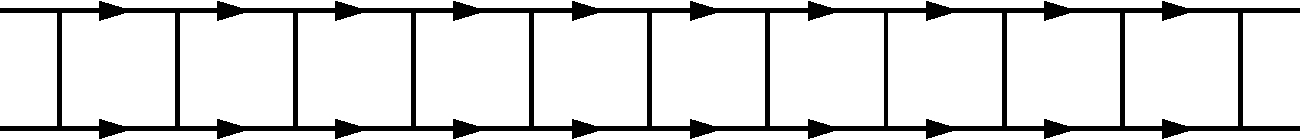
\includegraphics[width=0.85\linewidth]{figures/chapterNotation/fig1}
		
		\caption{Part of the Cayley graph for $
			\left\langle
			t,a
			\, \middle\vert \,
			a^2 = 1,\,
			ta = at
			\right\rangle
			$.}
		\label{fig:cg1}
	\end{figure}

	Performing the substitution $c = at$, the presentation
	$
	  G =
	  \left\langle
	  c,t
	  \, \middle\vert \,
	  c^2 = t^2 = 1,
	  ct = tc
	  \right\rangle
	$
	can be obtained, resulting in the Cayley graph shown in \cref{fig:cg2}.
	
	\begin{figure}[h!]
		\centering
		
		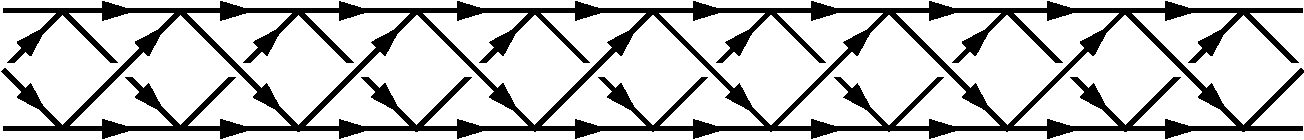
\includegraphics[width=0.85\linewidth]{figures/chapterNotation/fig2}
		
		\caption{Part of the Cayley graph for $  \left\langle
		  c,t
		  \, \middle\vert \,
		  c^2 = t^2 = 1,
		  ct = tc
		  \right\rangle$.}
		\label{fig:cg2}
	\end{figure}

	Notice that, by inspection of the two Cayley graphs, the group has polynomial geodesic growth with respect to the generating set $\left\lbrace t,a \right\rbrace$, and exponential geodesic growth with respect to the generating set $\left\lbrace c,t \right\rbrace$.
	More precisely, the group has geodesic growth $2n+2$  with respect to the generating set $\left\lbrace t,a \right\rbrace$, and geodesic growth of $2^n$  with respect to the generating set $\left\lbrace c,t \right\rbrace$.
\end{example}

\begin{example}[Example 6 from \cite{OnGroupsPolynomial}]
	A simpler example of this can be obtained by adding redundant generators to a group presentation. For example, the group formed by the integers with addition, $\mathbb{Z}$, with the usual presentation, $\left\langle z \, \middle\vert - \right\rangle$, and generating set, $\left\lbrace z \right\rbrace$, has a polynomial geodesic growth rate of $2n+1$.
	Then, by adding a redundant generator, $t$, the presentation $\left\langle z,t \middle\vert \, t = z  \right\rangle$ may be obtained, which has an exponential geodesic growth rate of $2 \cdot 2^n + 1$.
\end{example}

\begin{remark}
	Thus, by considering the previous example along with \cref{rmk:differentGrowthClasses}, it can be seen that the geodesics growth function $\gamma_{G,X}$ can vary in complexity under change of generating set.
	\thmendmark
\end{remark}

By the definition of $X$ as a generating set for $G$, it is known that for every element $g \in G$ there is at least one word $w \in \left( X \cup X^{-1} \right)^\ast$ such that $g = \overline{w}$.
Thus, the following proposition follows.

\begin{proposition}
	\label{prop:growth-function-bounds}
	The geodesic growth functions $S_{G,X}$ and $\Gamma_{G,X}$ are bounded from below by the growth functions $s_{G,X}$ and $\gamma_{G,X}$, respectively.
	Thus, both $s_{G,X} \preccurlyeq S_{G,X}$ and $\gamma_{G,X} \preccurlyeq \Gamma_{G,X}$.
\end{proposition}

\section{Intermediate Growth}
\label{sec:interGrowth}

The following definitions have been adapted from \cite{GrigPak} and \cite{HowGroupsGrow}.

Within this thesis, growth function will often be referred to as being polynomial, exponential or intermediate.
This section will define these terms with respect to the equivalence relation, $\sim$, from \cref{def:GrowthEquivRel} and the order, $\preccurlyeq$, from \cref{def:GrowthTotalOrd}.
In the following, let $f : \mathbb{N} \to \mathbb{N}$ be some arbitrary cumulative growth or cumulative geodesic growth function.

\begin{definition}
	The function $f$ is called \emph{polynomial} if there exists some $\alpha > 0$ such that $f \preccurlyeq n^\alpha$.
\end{definition}

\begin{definition}
	The function $f$ is called \emph{exponential} if $f \sim e^n$.
	\thmendmark
\end{definition}

Let $X$ be the finite generating set for the group, $G$, of which $f$ is a growth function.
Then, with $m = \left\vert X \right\vert\geq 1$, it can be seen that there can be no more than $(2m)^n$ words of length $n$ in the language $\left( X \cup X^{-1} \right)^\ast$.
Thus, there can be no more than $(2m)^n$ elements in $G$ of length $n$.
Hence,
\[
  f(n) \leq
  (2m)^0 + (2m)^1 + \cdots + (2m)^n
  \leq
  (2m)^{n+1}
\]
Thus, $f$ is always bounded from above by an exponential $(2m)^{n+1}$.

Therefore, $f$ is at most exponential in growth type, that is, $f \preccurlyeq e^n$.

Then, a growth function $f$ of \emph{intermediate growth} can be defined as one that is neither polynomial nor exponential.
To make this definition more convenient, the terms superpolynomial (a function which grows faster than any polynomial) and subexponential (a function that grows strictly slower than any exponential) will be defined; a function of intermediate growth will then be defined as one that is both superpolynomial and subexponential.

Firstly, the following lemma of cumulative growth functions will be shown.

\begin{lemma}
	The value of the limit \[ d(f) \coloneqq \limsup_{n \to \infty} \frac{\log f(n)}{\log n} \] known as the \emph{degree} of $f$, exists and lies in $\mathbb{R}_{\geq 0} \cup \left\lbrace \infty \right\rbrace$.
\end{lemma}

\begin{proof}
	Every value $\log f(n) / \log n$ of the sequence is non-negative, thus, considering that the limit superior is defined in $\mathbb{R}\cup \lbrace \pm \infty \rbrace$ for any sequence of reals, then the limit $d(f)$ exists and $d(f)\geq 0$.
	Therefore, $d(f)$ lies in $\mathbb{R}_{\geq 0} \cup \left\lbrace \infty \right\rbrace$ as required.
\end{proof}

Then, the degree $d(f)$ can be used to describe polynomial functions as follows.

\begin{proposition}
	The function $f$ is polynomial if and only if $d(f)$ is finite.
\end{proposition}

\begin{proof}
	\ \\
	$(\Longrightarrow)$
	Suppose that $f \preccurlyeq n^\alpha$, and thus there exists a constant $C \in \mathbb{N}_+$ such that $f(n) \leq C \cdot (C \cdot n)^\alpha$ for every $n \in \mathbb{N}_+$.
	Then, it follows that
	\[
	  \frac{\log f(n)}{\log n}
	  \leq
	  \frac{\log\left(C \cdot (C \cdot n)^\alpha\right)}{\log n}
	  =
	  \frac{\alpha \cdot \log n + (1+\alpha) \log C}{\log n}
	  =
	  \alpha + \frac{(1+\alpha) \log C}{\log n}
	\]
	Then, $d(f) \leq \alpha$ since $(1+\alpha)\log(C)/\log n \to 0$ as $n \to \infty$.
	Therefore, $d(f)$ is finite as required.
	
	$(\Longleftarrow)$
	Suppose that $d(f) = \beta < \infty$.
	Then, for $N \in \mathbb{N}$ sufficiently large,
	\[
	  \frac{\log f (n)}{\log n} \leq \beta + 1
	  \qquad
	  \text{for all}
	  \quad
	  n > N
	\]
	Letting $\alpha = \beta + 1$, it follows that for each $n > N$
	\[
	  \frac{\log f (n)}{\log n}
	  \leq \alpha
	  \quad
	  \Longrightarrow
	  \quad
	  \log f(n) \leq \alpha \cdot \log n
	  \quad
	  \Longrightarrow
	  \quad
	  f(n) \leq n^\alpha
	\]
	Thus, $f(n) \leq f(N) \cdot n^{\alpha}$ for all $n \in \mathbb{N}_+$.
	Therefore, $f(n) \preccurlyeq n^{\alpha}$ and is thus polynomial as required.
\end{proof}

From the previous proposition, the following definition results.

\begin{definition}
	\label{def:superpolynomial}
	The function $f$ is called \emph{superpolynomial} if $d(f) = \infty$.
	\thmendmark
\end{definition}

Now, the following lemma will be used to define subexponential growth rates.

\begin{lemma}[Grigorchuk-Pak \cite{GrigPak}]
	\label{lemma:growth-rate-bound}
	The limit
	\[
	  \omega(f) \coloneqq \lim_{n \to \infty} \frac{\log f(n)}{n}
	\]
	known as the \emph{growth rate} of $f$, always exists and has its value in $\mathbb{R}_{\geq 0}$.
	\thmendmark
\end{lemma}

The growth rate, $\omega(f)$ can then be related to the exponential growths as follows.

\begin{proposition}
	The function $f$ is exponential if and only if $\omega(f) > 0$.
\end{proposition}

\begin{proof}
	\ \\
	$(\Longrightarrow)$
	Suppose that $e^n \preccurlyeq f$, and thus there exists a constant $C \in \mathbb{N}_+$ such that $e^n \leq C \cdot f(C\cdot n)$ for all $n \in \mathbb{N}_+$.
	Then, it follows that
	\[
	  \frac{\log\left( C \cdot f(C \cdot n) \right)}{C n}
	  \geq
	  \frac{\log \left(e^n\right)}{Cn}
	  =
	  \frac{1}{C}
	\]
	Hence,
	\[
	  \frac{\log f(C \cdot n) }{Cn}
	  \geq
	  \frac{1}{C}
	  - \frac{\log C}{Cn}
	\]
	for each $n \in \mathbb{N}_+$.
	Notice that $\log C / Cn \to 0$ as $n \to \infty$.\\
	Therefore, $\omega(f) \geq 1/C > 0$ and thus $\omega(f)>0$ as required.
	
	$(\Longleftarrow)$
	Suppose that $w(f) = \beta > 0$, then for $N \in \mathbb{N}$ sufficiently large,
	\[
	  \frac{\log f(n)}{n}
	  \geq
	  \frac{\beta}{2}
	  \qquad
	  \text{for all}
	  \qquad
	  n > N
	\]
	Then, letting $\alpha = \beta/2$ it follows that $f(n) \geq e^{\alpha n} $ for all $n > N$.
	Thus, $f(n) \geq f(N) \, e^{\alpha n}$ for every $n \in \mathbb{N}_+$ and therefore $e^n \preccurlyeq f$.
	
	Then since $f \preccurlyeq e^n$, which was shown earlier in this section, it follows that $f \sim e^n$ as required.
\end{proof}

From this proposition, the following definition results.

\begin{definition}
	\label{def:subexponential}
	The function $f$ is called \emph{subexponential} if $\omega(f) = 0$.
	\thmendmark
\end{definition}

Thus, the class of intermediate growth functions can be defined as followed.

\begin{definition}
	The function $f$ is of \emph{intermediate growth} if it is both superpolynomial and subexponential as in \cref{def:superpolynomial,def:subexponential}, respectively.
\end{definition}

\begin{example}
	The function $e^{\sqrt{n}}$ is an example of intermediate growth.
	For an example of a particular group with intermediate growth, one can consider Grigorchuk's first group which was first defined by Grigorchuk in \cite{GrigFirst} and later proven to have intermediate growth in \cite{GrigInterm};
	in particular, Grigorchuk showed that this group possesses a cumulative growth $\gamma$ with
	\[
	  e^{\displaystyle \sqrt{n}}
	  \preccurlyeq
	  \gamma
	  \preccurlyeq
	  e^{\displaystyle n^{\log_{32} (31) }}
	\]
	which implies that $\gamma$ is of intermediate growth.
\end{example}




\chapter{Fabrykowski-Gupta Group}
\label{chp:FG-group}

The following definition of the Fabrykowski-Gupta group has been taken from \cite{OnGrowth}.

Let $A = \mathbb{Z}/3\mathbb{Z}$ be the finite additive group of order three, $\mathcal{T}_3$ denote the regular ternary tee $A^\ast$ with root $\varepsilon$, and let $t$ and $z$ be automorphisms of the tree $\mathcal{T}_3$ where $t$ cyclically permutes the first level of the tree, and the action of $z$ is defined recursively as $z = \recurDef{ t, 1 , z }$.
Thus, if $a \in A$ and $w \in A^\ast$ then,
\begin{align*}
	t \cdot (aw) &= ((a + 1)\text{ mod }3) \, w,
	&
	z \cdot (0w) &= 0 \, (t \cdot w),
	&
	z \cdot (1w) &= 1 \, w,
	&
	z \cdot (2w) &= 2 \, (z \cdot w)
\end{align*}
A group whose elements can be defined recursively as actions on a rooted regular tree in this way is called \emph{self-similar}.
More precisely, a group $G$ is said to be self-similar if its elements can be viewed as faithful actions of some tree $B^\ast$, where $B$ is a set; and for any $g\in G$ and $b\in B$, there exists a $h \in G$ and $b^\prime \in B$ such that $g \cdot (bx) = b^\prime \left(h \cdot x\right)$ for every $x \in B^\ast$.
Given such a group, the word \emph{restriction} of $g\in G$ to $b\in B^\ast$, denoted $\left. g \right\vert_b$, is the group element $h \in G$ such that $g \cdot (b x) = b^\prime \left( h\cdot x \right)$ for every $x \in B^\ast$ where $b^\prime \in B^\ast$ and $\left\vert b \right\vert = \left\vert b^\prime \right\vert$.
That is, the restriction $\left. g \right\vert_b$ is the action that $g \in G$ performs on the node corresponding to $b\in B^\ast$ of the tree

The actions of $t$ and $z$ can also be viewed geometrically as in the following figure.

\begin{figure}[!ht]
	\centering

	\begin{subfigure}[b]{.48\linewidth}
		\centering
		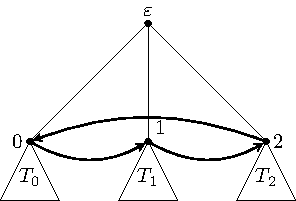
\includegraphics{figures/groupActions/tAction}
		\caption{action of $t$}
		\label{fig:action-t}
	\end{subfigure}
	\hfill
	\begin{subfigure}[b]{.48\linewidth}
		\centering
		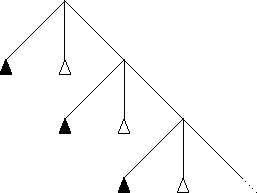
\includegraphics{figures/groupActions/zAction}
		\caption{action of $z$}
		\label{fig:action-z}
	\end{subfigure}

	\caption{Actions of $t$ and $z$ on $\mathcal{T}_3$}
	\label{fig:actions}
\end{figure}

In \cref{fig:action-t}, the first level of the tree is cyclically permuted, and the sub-trees $T_0$, $T_1$ and $T_2$ are fixed i.e.\ not permuted.
In \cref{fig:action-z}, the solid triangles, \tActionNotation, denote that an action of $t$ is taken on the associated sub-tree; and the hollow triangles, \idActionNotation, indicate that the associated sub-tree is fixed.

The \emph{Fabrykowski-Gupta group} is the group generated by the actions $t$ and $z$ as described earlier.

\begin{notation}
	Let $\mathbb{G} = \left\langle t, z \right\rangle$ denote the Fabrykowski-Gupta group
	\thmendmark
\end{notation}

Considering the geometric definition of the actions $t$ and $z$ given in \cref{fig:actions}, it can be seen that both $z^3$ and $t^3$ are equivalent to the identity as they fix $\mathcal{T}_3$.
Thus, elements of the Fabrykowski-Gupta group can be represented as alternating words of $t^{\pm 1}$ and $z^{\pm 1}$.
That is, words of the form
\begin{align*}
	\left(t^{\varepsilon_1}\right)\, z^{\delta_1}\,
	t^{\varepsilon_2}\, z^{\delta_2}\,
	\cdots
	t^{\varepsilon_n}\, z^{\delta_n}\,
	\left(t^{\varepsilon_{n+1}}\right)
\end{align*}
where each $\varepsilon_i, \delta_i \in \left\lbrace -1,1 \right\rbrace$, and the brackets, $(\cdot)$, indicate that the first and last $t^{\varepsilon_j}$ are optional.
This will be known as the \emph{alternating form} of words in the Fabrykowski-Gupta group.

Let $\Stab(1)$ be the subgroup of $\mathbb{G}$ that stabilises the first level of the tree $\mathcal{T}_3$, that is, the subgroup which doesn't permute the first level.
Notice that $\Stab(1)$ is generated by
\begin{align*}
	z_0 = z &= \recurDef{ t,1,z },
	&
	z_1 = z^t &= \recurDef{ z,t,1 },
	&
	z_2 = z^{t^{-1}} &= \recurDef{ 1,z,t }
\end{align*}
That is,
\[
\Stab(1) = \left\langle z_0, z_1, z_2 \right\rangle
\]
Thus, the Fabrykowski-Gupta group can be written as the semidirect product $\Stab(1) \rtimes \left\langle t \right\rangle$.
Therefore, every element of the Fabrykowski-Gupta group can be written in the form
\[
	\tau
	\,
	z_{c_1}^{\varepsilon_1}
	\,
	z_{c_2}^{\varepsilon_2}
	\cdots
	z_{c_n}^{\varepsilon_n}
	\quad
	\text{where}
	\quad
	c_i \in \left\lbrace 0,1,2 \right\rbrace,\ 
	\varepsilon_i \in \left\lbrace -1,1 \right\rbrace
	\text{ and }
	\tau \in \left\lbrace 1,t,t^{-1} \right\rbrace
\]
This will be known as the \emph{coset form} of words in the Fabrykowski-Gupta group.

\begin{remark}
	Neither the alternating form nor the coset form, as described earlier, represent elements in the Fabrykowski-Gupta group uniquely.
	Thus, neither of these forms are normal forms.
	The purpose and relevance of these two forms will become apparent in the following sections.
\end{remark}

\begin{note*}
	In subsequent sections of this chapter $X$ will denote the symmetric generating set of the Fabrykowski-Gupta group, that is, $X = \left\lbrace t^{\pm 1}, z^{\pm 1}\right\rbrace$.
\end{note*}

\section{Forms of Words}

This section will introduce some properties of the alternating and coset form, both of which ere defined previously in this chapter.

\begin{proposition}
	\label{prop:geodesics-in-alt-form}
	All geodesics of the Fabrykowski-Gupta group are in the alternating form.
\end{proposition}

\begin{proof} Let $w\in X^*$ be a word that is not in the alternating form.
	
	%Since $w$ is not in the alternating form, 
	Then either $w$ is not freely reduced or contains a subword $t^2$, $t^{-2}$, $z^2$ or $z^{-2}$;
	thus, a strictly shorter word $w^\prime$ can be obtained by either freely reducing $w$ or replacing one of the aforementioned subwords with $t^{-1}$, $t$, $z^{-1}$ or $z$, respectively. 
	
	Notice that the word $w^\prime$ and $w$  will correspond to the same group element.
	
	Thus, $w$ is not geodesic as there is a strictly shorter word $w^\prime$ that represents the same element.
\end{proof}

It is known that every element of the Fabrykowski-Gupta group can be represented by a word in the coset form.
However, the process of generating such a representation may not be as obvious.
The process of taking a word from the alternating form to the coset form is a simple rewrite procedure in which the letters of the word are read right-to-left; to understand the idea of this procedure, consider the following example.

\begin{example}
	Consider the word $t^{-1} z t z^{-1} t z$, in the alternating form, as follows.
	\begin{align*}
	  t^{-1} z t z^{-1} t z
	  &\mapsto t^{-1} z t z^{-1} t \left(z\right)
	   &&\left(z\text{ is already in the coset form}\right)
	   \\
	  &\mapsto t^{-1} z t^{-1} \left( t^{-1}  z^{-1} t\right) \left(z\right)
	   &&\left(\text{replaced a }t\text{ with }t^{-1}t^{-1}\right)
	   \\
	  &\mapsto t \left(t z t^{-1}\right) \left( t^{-1}  z^{-1} t\right) \left(z\right)
	   &&\left(\text{replaced a }t^{-1}\text{ with }tt\right)
	   \\
	  &\mapsto \left(t\right) \left(t z t^{-1}\right) \left( t^{-1}  z^{-1} t\right) \left(z\right)
	   &&\left(\text{only a }t\text{ remains}\right)
	   \\
	  &\mapsto t \, z_2 \, z_1^{-1} \, z_0
	   &&\left(\text{rewrite in the coset form}\right)
	\end{align*}
	Thus, it can be seen that $t^{-1} z t z^{-1} t z$ is equivalent to $t \, z_2 \, z_1^{-1} \, z_0$ in the coset form.
	\thmendmark
\end{example}

The previous example shows the idea of working from right-to-left over a word in the alternating form, matching conjugates of $z^{\pm 1}$ by replacing  $t$'s and $t^{-1}$ with $t^{-1}t^{-1}$ and $tt$, respectively, where necessary.
Considering this rewrite procedure, it can be seen that a word in the alternating form can be converted to the coset form in linear time with respect to word length of the input.
Thus, the following lemma results.

\begin{lemma}
	\label{lemma:coset-form-linear}
	A word $w \in X^\ast$ in the alternating form, can be converted to an equivalent word in the coset form in linear time with respect to the word length of $w$.
\end{lemma}

\begin{remark}
	\label{rmk:constantNumberZ}
	Notice that the previously described process does not replace or omit any $z$'s or $z^{-1}$'s.
	Thus, the word in the coset form obtained from the previously described procedure will have the same number of $z$'s and $z^{-1}$'s as the original word in the alternating form.
	\thmendmark
\end{remark}

The coset form is of interest as it allows for easy computation of word restrictions to the first level of the tree $\mathcal{T}_3$.
To compute these restrictions, the following maps will be defined.

\begin{definition}
	\label{def:phi-maps}
	Let the following maps $\phi_0$, $\phi_1$ and $\phi_2$  be defined as
	\begin{align*}
	\phi_0 &=
	\begin{cases}
	z_0 \mapsto t\\
	z_1 \mapsto 1\\
	z_2 \mapsto z
	\end{cases}
	&
	\phi_1 &=
	\begin{cases}
	z_0 \mapsto z\\
	z_1 \mapsto t\\
	z_2 \mapsto 1
	\end{cases}
	&
	\phi_2 &=
	\begin{cases}
	z_0 \mapsto 1\\
	z_1 \mapsto z\\
	z_2 \mapsto t
	\end{cases}
	\end{align*}
	where each $\phi_j$ maps $t \mapsto 1$ and preserved inverses.
	Now, define
	\[
	  \phi_j\left(
	    \tau
	    \,
	    z_{c_1}^{\varepsilon_1}
	    \,
	    z_{c_2}^{\varepsilon_2}
	    \cdots
	    z_{c_n}^{\varepsilon_n}
	  \right)
	  =
	  \phi_j\left(z_{c_1}^{\varepsilon_1}\right)
	  \phi_j\left(z_{c_2}^{\varepsilon_2}\right)
	  \cdots
	  \phi_j\left(z_{c_n}^{\varepsilon_n}\right)
	\]
	for each word $\tau \, z_{c_1}^{\varepsilon_1} \, z_{c_2}^{\varepsilon_2} \cdots z_{c_n}^{\varepsilon_n}$ in the coset form.
\end{definition}

\begin{proposition}
	\label{prop:word-restrictions}
	Given a word $w \in X^\ast$ in the coset form, the words $\phi_0(w)$, $\phi_1(w)$ and $\phi_2(w)$ are equivalent to the restrictions $\left. w \right\vert_0$, $\left. w \right\vert_1$ and $\left. w \right\vert_2$, respectively.
\end{proposition}

\begin{proof}
	This follows from the recursive definition of $z_0$, $z_1$ and $z_2$.
\end{proof}

\begin{proposition}
	\label{prop:phiLengthReduce}
	Given a word of length $n$, each of its restrictions to the first level, as computed by converting to the coset form then applying the appropriate map $\phi_j$, are of length at most $\left\lceil n / 2 \right\rceil$.
\end{proposition}

\begin{proof}
	This proof will first show the statement for words in the alternating form, and then extend it to all words in the language $X^\ast$.
	
	Let $w$ be a word in the alternating form of length $n$.\\
	Then, $w$ can contain at most $\left\lceil n/2 \right\rceil$ letters of the form $z^{\pm 1}$.
	
	Thus, by considering \cref{rmk:constantNumberZ}, it can be seen that the coset form of $w$, obtained by the earlier described procedure, can contain at most $\left\lceil n/2 \right\rceil$ letters of the form $z_j^{\pm 1}$ as each $z_j^{\pm 1}$ contains exactly one letter of the form $z^{\pm 1}$.
	
	Thus, by applying one of the maps $\phi_j$, a word of length at most $\left\lceil n/2 \right\rceil$ will be obtained.\\
	Thus, completing the proof for the case of words in the alternating form.
	
	To see that this result generalises to all words in the language $X^\ast$, let some word $w \in X^\ast$ of length $m$ be given.
	Then, by repeatedly performing free reduction and replacing occurances of $z^2$, $z^{-2}$, $t^{2}$ and $t^{-2}$ with $z^{-1}$, $z$, $t^{-1}$ and $t$, respectively, a word $w^\prime$ in the alternating form of length $n\leq m$ is obtained.
	
	By then applying the earlier argument of this proof to $w^\prime$, it can be seen that the first level restrictions of $w$ are of length at most $\left\lceil n / 2 \right\rceil \leq \left\lceil m / 2 \right\rceil$.
	Thus, completing the proof.
\end{proof}

A self-similar group $G$ that acts on a tree $B^\ast$ is said to be \emph{contracting} if there exists a finite set $\mathcal{N} \subset G$, called a \emph{nucleus}, such that for every element $g \in G$ there is an $N \in \mathbb{N}$ such that $\left. g \right\vert_b \in \mathcal{N}$ for every $b\in B^N$.
That is, the actions of $g$ on the $N$-th level of the tree $B^\ast$ are all in the set $\mathcal{N}$.
Notice that the aforementioned $N \in \mathbb{N}$ can be dependent on the element $g \in G$.

\begin{corollary}
	\label{cor:nucleus}
	Fabrykowski-Gupta is contracting with a nucleus of $\mathcal{N} = \left\lbrace 1, t^{\pm 1}, z^{\pm 1}\right\rbrace$.
\end{corollary}

\begin{proof}
	Let $w \in X^\ast$.
	Considering the previous proposition (\ref{prop:phiLengthReduce}), it can be seen that by an induction on the length of words, that there must exist some depth of the tree, $N$, for which all restrictions, $\left. w \right\vert_a$ with $a \in A^N$, to the $N$-th level are of word length $0$ or $1$.
	
	Thus, each of $\left. w \right\vert_a$ with $a\in A^N$ must be in the set $\mathcal{N}$ as this is the set of all words of length $0$ and $1$.
	
	Hence, Fabrykowski-Gupta is contracting with a nucleus of $\mathcal{N}$.
\end{proof}

From \cref{lemma:coset-form-linear}, it is known that a word can be converted from the alternating form to the coset form in linear time.
It is also true that any word in the language $X^\ast$ can be converted to the alternating form in linear time with respect to the word length of the input word.
To see this, let some word $w \in X^\ast$ in the alternating form be given.
Then, given some letter $a \in X$, the word $wa$ can be computed in the alternating form by considering the following two cases:
\begin{itemize}
	\item[(1)] If $w$ does not end in $a$ or $a^{-1}$ then simply concatenating the $a$ to the end of $w$ will result in a word in the alternating form;
	\item[(2)] If $w$ ends in $a$ or $a^{-1}$, then replace this letter with $a^{-1}$ or remove it, respectively.
\end{itemize}
Thus, appending a letter to a word in the alternating form, obtaining a result in the alternating form, can be done in constant time.

Hence, a word $w\in X^\ast$ of length $n = \left\vert w \right\vert$ can be converted to the alternating form by reading $w$ from left-to-right, appending its letters to a word $v$ in the alternating form to obtain a word in the alternating form.
Thus, if $v$ is initially the empty word, then after $n$ steps of a constant time procedure $v$ will contain an equivalent word in the alternating form.
Thus, the following results.

\begin{lemma}
	\label{lemma:alt-form-linear}
	A word $w \in X^\ast$ can be converted to an equivalent word in the alternating form in linear time with respect to the word length of $w$.
\end{lemma}

%\newpage
\section{Word Problem}
\label{sec:word-problem}

This section presents an efficient algorithm which solves the word problem for the Fabrykowski-Gupta group.
The details and complexity analysis of this algorithm will be provided as it is used by the brute force algorithm for generating geodesics, which will be described in the next chapter.
The purpose of this section is to show that the word problem, in the case of Fabrykowski-Gupta, is solvable in time $O(n \log n)$ with respect to the word length of input words.

The algorithm described in this section relies heavily on the maps $\phi_j$, as described in \cref{def:phi-maps,prop:word-restrictions}, to compute the restrictions of words.
The complexity of this algorithm will then be proven by the use of \cref{lemma:coset-form-linear,lemma:alt-form-linear,prop:phiLengthReduce,prop:word-restrictions,cor:nucleus}.

For the purpose of this section, unless otherwise specified, let $w \in X^\ast$ be some arbitrary word.

Considering that $w$ is equivalent to the identity of $\mathbb{G}$ if and only if its action fixes every node of the tree $\mathcal{T}_3$, then it can be seen that the word problem may be solved recursively as given in \cref{alg:word-problem} on the following page.

\begin{algorithm}[!ht]
	
	\Fn(){\WP{$w$}}{
		\KwData{an input word $w \in X^\ast$}
		\KwResult{true if and only if $w$ is equivalent to the identity}
		
		\BlankLine
		
		Convert $w$ to the alternating form\;
		\label{alg:word-problem:convert-to-alt}
		
		\BlankLine
		
		\If{$\left\vert w \right\vert = 0$}{
			\label{alg:word-problem:check-trivial}
			\Return{true}\tcc*{$w$ is the empty word}
		}
	
		\BlankLine
	
		\If{$\left\vert w \right\vert = 1$} {
			\label{alg:word-problem:check-generator}
			\Return{false}\tcc*{$w$ represents a generator}
		}
	
		\BlankLine
	
		\If{$w$ permutes the first level of $\mathcal{T}_3$}{
			\label{alg:word-problem:check-first-level}
			\Return{false}\tcc*{$w$ permutes the first level}
		}
	
		\BlankLine
	
		Convert $w$ to the coset form\;
		\label{alg:word-problem:convert-coset}
		
		\BlankLine
		
		\tcp{check the action on the left sub-tree}
		
		$v \gets \phi_0(w)$\;
		\label{alg:word-problem:left-rist}
		
		\If{\WP{$v$} $=$ false}{
			\label{alg:word-problem:left-rec}
			\Return{false}\tcc*{$w$ permutes the left sub-tree}
		}
	
		\BlankLine
	
	    \tcp{check the action on the middle sub-tree}
	    
		$v \gets \phi_1(w)$\;
		\label{alg:word-problem:middle-rist}
		
		\If{\WP{$v$} $=$ false}{
			\label{alg:word-problem:middle-rec}
			\Return{false}\tcc*{$w$ permutes the middle sub-tree}
		}
	
		\BlankLine
		
		\tcp{check the action on the right sub-tree}
	
		$v \gets \phi_2(w)$\;
		\label{alg:word-problem:right-rist}
		
		\If{\WP{$v$} $=$ false}{
			\label{alg:word-problem:right-rec}
			\Return{false}\tcc*{$w$ permutes the right sub-tree}
		}
	
		\BlankLine
	
		\Return{true}\tcc*{$w$ does not permute the first level or any sub-tree}
		\label{alg:word-problem:final-return}
	}
	
	\caption{Word Problem}
	\label{alg:word-problem}
\end{algorithm}

The idea of this algorithm is to first check that the action of $w$ fixes the first level of the tree $\mathcal{T}_3$, then recursively check that it fixed any of the sub-trees.
For this algorithm to be valid, it remains to be shown that it will terminate on any given input; to see this, consider the following theorem which shows an upper bound on the complexity of \cref{alg:word-problem}.

%\newpage
\begin{theorem}
	\label{thm:word-problem-complexity}
	\Cref{alg:word-problem} has a time complexity of $O(n\log n)$.
\end{theorem}

\begin{proof}

Let $n$ be the size of the input word i.e.\ $n = \left\vert w \right\vert$.

From \cref{prop:phiLengthReduce}, it can be seen that \cref{alg:word-problem} will only consider word restrictions down to a maximum depth of $\left\lceil \log_2 n \right\rceil$.
This is clear as at this depth, all word restrictions, as computed by appropriate applications of the maps $\phi_j$, will be of length $0$ or $1$, and thus \cref{alg:word-problem} will be able to return either `true' or `false' at, or before, this depth is reached.

Now, consider the complexity of each of the lines of the algorithm.
From \cref{lemma:alt-form-linear}, it is known that words can be converted to the alternating form in linear time, and thus \cref{alg:word-problem:convert-to-alt} will run in linear time; also and after this line $w$ can't increase in word length.
It is clear that a word's action on the first level of $\mathcal{T}_3$ can be checked in linear time (simply by considering the $t$'s and $t^{-1}$'s in $w$), and thus \cref{alg:word-problem:check-first-level} will run in linear time.
From \cref{lemma:alt-form-linear} it is known that words in the alternating form can be converted to the coset form in linear time, and thus \cref{alg:word-problem:left-rist,alg:word-problem:middle-rist,alg:word-problem:right-rist} will run in linear time.
All the remaining lines, except for the recursive calls on \cref{alg:word-problem:left-rec,alg:word-problem:middle-rec,alg:word-problem:right-rec}, will run in constant time.

Therefore, every line of \cref{alg:word-problem}, except for the recursive calls on \cref{alg:word-problem:left-rec,alg:word-problem:middle-rec,alg:word-problem:right-rec}, will run within linear time with respect to the size, $n$, of the input word.

Let $\#_z : X^\ast \to \mathbb{N}$ count the number of $z$'s and $z^{-1}$'s in a word.
For example, $\#_z\left(tztz^{-1}t^{-1}\right) = 2$.

In the remainder of this proof, let $\left. w \right\vert_a$ denote the word restriction of $w$ to $a$ as calculated by an appropriate sequence of applications of the maps $\phi_j$.

Now, considering the maps $\phi_j$, as given in \cref{def:phi-maps}, it can be seen that the following inequality holds for $w$ in the alternating form
\[
\#_z(w) \geq
\#_z\left(\left. w \right\vert_0 \right) +
\#_z\left(\left. w \right\vert_1 \right) +
\#_z\left(\left. w \right\vert_2 \right)
\]
Hence by induction, for any depth, $m$, of the tree $\mathcal{T}_3$ then,
\[
\#_z(w) \geq
\sum_{a \in A^m}
\#_z\left(\left. w \right\vert_a \right)
\]
where $m \in \mathbb{N}$ is a depth of the tree $\mathcal{T}_3$.

Now considering again the maps $\phi_j$, and the recursive definition of $z$ as $\recurDef{t,1,z}$, it can be seen that the total word length of the restrictions to the $m$-th level of $\mathcal{T}_3$ can be no more than two times the total number of $z$'s and $z^{-1}$'s in the word restrictions on the $(m-1)$-th level, that is,
\[
  \sum_{a \in A^{m}}
  n_a
  \leq
  2
  \sum_{a \in A^{m-1}} \#_z\left(\left. w \right\vert_a \right)
\]
where $n_a$ is the word length of the restriction $\left. w \right\vert_a$.
Thus, for $m > 0$,
\[
  \sum_{a \in A^{m}}
  n_a
  \leq
  2
  \cdot
  \#_z(w)
\]
Further, with $w$ in the alternating form, it follows that $\#_z(w)$ can be no more than $\left\lceil n/2 \right\rceil$ where $n$ is the word length of $w$.
Thus,
\[
  \sum_{a \in A^{m}}
  n_a
  \leq
  2
  \left\lceil n/2 \right\rceil
  \ \ 
  \text{for all }
  m > 0
  \text{, and thus,}
  \ \ 
  \sum_{a \in A^{m}}
  n_a
  \leq
  n+1
  \ \ 
  \text{for all levels }m \in \mathbb{N}\text{ of }\mathcal{T}_3.
\]
Thus, for each level $m \in \mathbb{N}$ of the tree $\mathcal{T}_3$, a linear time algorithm (i.e.\ everything except the recursive calls of \cref{alg:word-problem:left-rec,alg:word-problem:middle-rec,alg:word-problem:right-rec}) will be run $\ell$ times on inputs of word length $n_1$, $n_2$, \ldots, $n_\ell$, respectively, where $n_1 + n_2 + \cdots + n_\ell \leq n+1$.
Notice that instances where the algorithm is run with input of word length zero can be ignored as their run-times are constant and can be considered a part of the run-time of their respective callers.

Thus, \cref{alg:word-problem} is composed of no more than $\left\lceil \log_2 n \right\rceil$ instances (one for each level) of an algorithm of complexity $O(n)$.
Hence, the complexity of \cref{alg:word-problem} is $ O(\left\lceil \log_2 n \right\rceil n)$.

Therefore, the complexity of \cref{alg:word-problem} is $O(n \log n)$ as required.
\end{proof}

%\newpage
\section{Signatures}

This section will introduce three functions known which will be known as the signatures.
These functions were originally designed with the intention of improving the run-time of the brute force geodesic generating algorithm, which will be presented in \cref{sec:growth-functions}, by a constant factor.
However, these functions later became important when defining an algorithm, which will be presented in the next section, to compare words of the Fabrykowski-Gupta group.

This section will begin by defining the functions $\sig_t,\sig_z : X^\ast \to \left\lbrace 0, 1, 2 \right\rbrace$ which will be known as the $t$ and $z$ signatures, respectively.
These signatures will then be shown to be homomorphisms when considered as maps $\mathbb{G} \to (\mathbb{Z}/3\mathbb{Z}, +)$, and thus for any two words $w,v \in X^\ast$ with $w =_\mathbb{G} v$, it follows that $\sig_t(w) = \sig_t(v)$ and $\sig_z(w) = \sig_z(v)$.

Let some $w \in X^\ast$ be chosen, then the signatures $\sig_t(w)$ and $\sig_z(w)$ are defined as follows.

\begin{definition}
	\label{def:t-signature}
	The \emph{$t$-signature} of $w$, denoted $\sig_t(w)$, is the sum of powers of $t$ in $w$ modulo 3.
\end{definition}

\begin{example}
	To understand the $t$-signature, consider the following examples.
	\begin{align*}
	  \sig_t\left( z^n \right)         &= 0,             &
	  \sig_t\left( t^nzt^{-m} \right)         &\equiv (n-m) \mod 3, &
	  \sig_t\left( t^{-1}z t^2 \right) &= 1
	\end{align*}
\end{example}

\begin{definition}
	\label{def:z-signature}
	The \emph{$z$-signature} of $w$, denoted $\sig_z(w)$, is the sum of powers of $z$ in $w$ modulo 3.
\end{definition}

\begin{example}
	To understand the $z$-signature, consider the following examples.
	\begin{align*}
	\sig_z\left( z^n \right)     &\equiv n \mod 3, &
	\sig_z\left( t^n \right)     &= 0,             &
	\sig_z\left( z t z^{-1}\right) &= 0
	\end{align*}
	\thmendmark
\end{example}

Notice that the signature $\sig_t(w)$ indicates how the word $w$ permutes the first level of the tree $\mathcal{T}_3$, that is, $\sig_t(w)$ is; $0$ if $w$ fixes the first level; $1$ if $w$ performs $t$ to the first level; and $2$ if $w$ performs $t^{-1}$ to the first level.
Then, since words which represent the same group element permute the first level in the same way, it follows that two such words have the same $t$-signature.
Thus, the $t$-signatures can be viewed as a map from $\mathbb{G}$ to the group $\left\langle t \, \middle\vert \, t^3 \right\rangle \cong (\mathbb{Z}/3\mathbb{Z},+)$.
Further, it can be seen that this map is in fact a homomorphism by considering the way in which words are composed.
Thus, the following proposition follows.

\begin{proposition}
	The $t$-signature function can be seen to be a homomorphism when viewed as a function which maps $\mathbb{G} \to (\mathbb{Z}/3\mathbb{Z},+)$.
	\thmendmark
\end{proposition}

It will now be shown that the $z$-signature function is also a homomorphism when taken to be a map $\mathbb{G} \to (\mathbb{Z}/3\mathbb{Z},+)$.
To do this, it will first be shown that $\sig_z(w) = 0$ whenever $w$ is equivalent to the identity. Now, considering the definition of the maps $\phi_j$ in \cref{def:phi-maps}, and \cref{prop:word-restrictions}, it can be seen that
\[
  \sig_z(w)
  \equiv
  \sig_t(\left. w \right\vert_0) +
  \sig_t(\left. w \right\vert_1) +
  \sig_t(\left. w \right\vert_2)
  \pmod{3}
\]
where each $\left. w \right\vert_j$ is calculated by the corresponding $\phi_j$ map.
Then, since $w$ is equivalent to the identity, it follows that each of the $\sig_t(\left. w \right\vert_j)$ it the above must be zero, and hence, $\sig_z(w) \equiv 0 \pmod{3}$.
Therefore, $\sig_z$ maps every word which is equivalent to the identity to zero as required.

Now, considering the way in which word inverses are calculated and concatenation of words, it can be seen that $\sig_z(w) + \sig_z(w^{-1}) = 0$ and $\sig_z(wv) = \sig_z(w) + \sig_z(v) \pmod{3}$ for all $w,v\in X^\ast$.
Let $w,v\in X^\ast$ be words such that $w =_\mathbb{G} v$, then
\[
  0 = \sig_z(w v ^{-1}) = \sig_z(w) - \sig_z(v)
\]
and thus, $\sig_z(w) = \sig_z(v)$.
Thus, $\sig_z$ can be viewed as a map from $\mathbb{G}$ to $(\mathbb{Z}/3\mathbb{Z},+)$ that preserves the group structure.
Thus, the following proposition results.

\begin{proposition}
	The $z$-signature function can be seen to be a homomorphism when viewed as a function which maps $\mathbb{G} \to (\mathbb{Z}/3\mathbb{Z},+)$.
	\thmendmark
\end{proposition}

For the purpose of convenience, the following additional signature will be defined.

\begin{definition}
	\label{def:full-signature}
	The \emph{full-signature} of $w$, denoted $\sig(w)$, is defined as
	\[
	  \sig(w) \coloneqq 3\cdot\sig_z(w) + \sig_t(w)
	  \in \left\{ 0,1,2,\ldots, 8 \right\}
	\]
	Thus, $\sig(w)$ can be viewed as a homomorphism $\mathbb{G} \to (\mathbb{Z}/3\mathbb{Z},+)^2$,
	where the elements of the form $(i,j) \in (\mathbb{Z}/3\mathbb{Z},+)^2$ are represented by the corresponding integers $(3\cdot i) + j$.
	Further, it can be seen that both $\sig_t(w)$ and $\sig_z(w)$ are recoverable from $\sig(w)$.
\end{definition}

\begin{remark}
	The full-signature of a word is represented as an integer in $\left\lbrace 0, 1, 2,\ldots, 8 \right\rbrace$, rather than a tuple of the form $\left\lbrace 0,1,2 \right\rbrace^2$, as this form becomes convenient when defining the word comparison algorithm of the next section.
\end{remark}

\begin{remark}
	Elements of the nucleus, $\mathcal{N} = \left\lbrace 1, t^{\pm 1}, z^{\pm 1} \right\rbrace$, are each assigned a different value by $\sig$, and thus elements of the nucleus are recoverable from their corresponding full signatures.
\end{remark}

\section{Comparing Words}
\label{sec:comparing-words}

This section will describe an algorithm that can compare any two words in the Fabrykowski-Gupta group in the sense that, given two words $w,v\in X^\ast$, then exactly one of $w < v$, $v < w$ or $w =_\mathbb{G} v$ will be true where $<$ is taken with respect to the comparison.
Further, this comparison algorithm will satisfy transitivity in the sense that, given some $u,v,w\in X^\ast$ such that $u < v$ and $v < w$, it follows that $u < w$.
This comparison algorithm then makes it possible to sort a list of words in the language $X^\ast$ with the use of a comparison-based sort algorithm.
This fact will be used in \cref{sec:sortingMethod} where it will be shown that the geodesics of the Fabrykowski-Gupta group may be generated efficiently by a modified sort algorithm.

The comparison algorithm described in this section is based on a variation of what are known as portraits.
A \emph{portrait} is a finite rooted tree where each node is decorated to shows how its corresponding sub-tree is permuted, and the leaves are decorated with an element of the group's nucleus.
For example, a portrait of the word $tztztztztz^{-1}t$ is given as in \cref{fig:tztztztztZtPortrait}.

\begin{figure}[!ht]
	\centering
	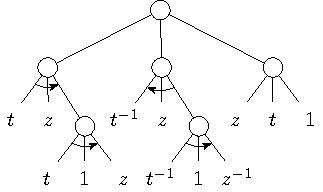
\includegraphics[width=.4\linewidth]{figures/portraits/tztztztztZtPortrait}

	\caption{A portrait of the word $tztztztztz^{-1}t$.}
	\label{fig:tztztztztZtPortrait}
\end{figure}

Notice that in \cref{fig:tztztztztZtPortrait} as above, an arrow from left-to-right indicates an action of $t$, an arrow from right-to-left indicated an action of $t^{-1}$, and the absence of an arrow indicated that the associated sub-tree is not cyclically permuted.
The action of a portrait should be read such that the actions of the leaves being applied first, followed by the arrows in a bottom-up order; the idea being that the action of the portrait is equivalent to the action of the corresponding group element.

Notice that any portrait can be written such that it's leaves are on the same level.
For example, \cref{fig:port2} shows an equivalent portrait for $tztztztztz^{-1}t$ (compare this with the previous portrait).

\begin{figure}[!ht]
\begin{center}
	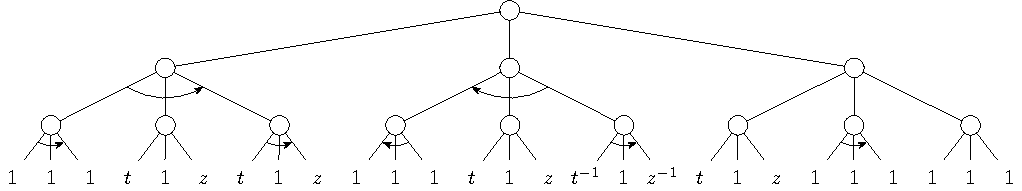
\includegraphics[width=\linewidth]{figures/portraits/tztztztztZtPortraitFull}
\end{center}
	\caption{A depth three portrait for $tztztztztz^{-1}t$.}
	\label{fig:port2}
\end{figure}

\begin{remark}
	Note that it is possible to define (finite) portraits in any contracting group.
	\thmendmark
\end{remark}

As was mentioned previously, the algorithm of this section is based on a modified version of these portraits.
In this modified version, which will be known as the \emph{signature portrait}, the finite trees are instead decorated with word signatures as in \cref{def:full-signature}.
For example, the words $z^{-1}tztzt$ and $z^{-1}tzt^{-1}zt^{-1}ztz^{-1}$ have the  (regular) portraits shown in \cref{fig:port3}. % respectively.

\begin{figure}[!ht]
	\centering
	
	\hfill
	\begin{subfigure}{.45\linewidth}
		\centering
		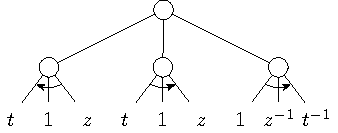
\includegraphics[width=\linewidth]{figures/portraits/ZtztztPortrait}
	\end{subfigure}
	\hfill
	\begin{subfigure}{.45\linewidth}
		\centering
		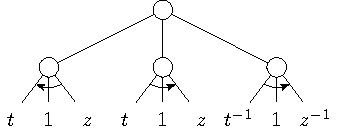
\includegraphics[width=\linewidth]{figures/portraits/ZtzTzTztZPortrait}
	\end{subfigure}
	\hfill

	\caption{(Regular) portraits for $z^{-1}tztzt$ and $z^{-1}tzt^{-1}zt^{-1}ztz^{-1}$, respectively.}
	\label{fig:port3}
\end{figure}

Now signature portraits of words $z^{-1}tztzt$ and $z^{-1}tzt^{-1}zt^{-1}ztz^{-1}$ are given in \cref{fig:port4}.

\begin{figure}[!ht]
\begin{center}
	
	\hfill
	\begin{minipage}{.45\linewidth}
		\centering
		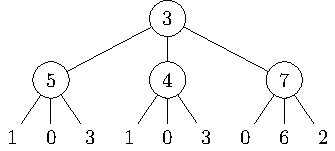
\includegraphics[width=\linewidth]{figures/portraits/ZtztztSigPortrait}
	\end{minipage}
	\hfill
	\begin{minipage}{.45\linewidth}
		\centering
		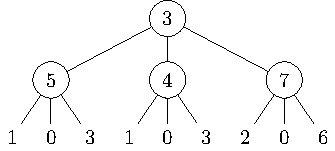
\includegraphics[width=\linewidth]{figures/portraits/ZtzTzTztZSigPortrait}
	\end{minipage}
	\hfill
	
\end{center}
\caption{Signature portraits for $z^{-1}tztzt$ and $z^{-1}tzt^{-1}zt^{-1}ztz^{-1}$, respectively}
	\label{fig:port4}
\end{figure}



Notice that in the signature portrait, the leaves must correspond to a node of the tree in which the word performs an action from the nucleus.
Also, the numbers on the leaves and nodes correspond to the value that `$\sig$' (see \cref{def:full-signature}) assigns to the corresponding word restrictions.

\begin{remark}
	A portrait is recoverable from each signature portrait; the elements on the leaves are recoverable as `$\sig$' assigns a different value to each element in the nucleus $\mathcal{N} = \left\lbrace 1,t^{\pm 1}, z^{\pm 1}\right\rbrace$; the arrows on the nodes are recoverable from the value of $\sig_t$ which is itself recoverable from  $\sig$.
	
	Hence, elements of the Fabrykowski-Gupta can be represented faithfully by signature portraits.
	\thmendmark
\end{remark}

Given two words $w,v \in X^\ast$, the idea of the comparison algorithm is to construct signature portraits for $w$ and $v$ of the same depths and to compare the trees in a depth-first order.
For example, the two signature portraits given earlier can be viewed as tuples $\mathbf{x} = (3,5,1,0,3,4,1,0,3,7,0,6,2)$ and $\mathbf{y} = (3,5,1,0,3,4,1,0,3,7,2,0,6)$, respectively, when the values are read in a depth-first order.
Notice that these tuples match in the first $10$ entries, but in the $11$-th entry $0 = \mathbf{x}_{11} < \mathbf{y}_{11} = 2$.
Hence, it is said that $\mathbf{x} < \mathbf{y}$, and thus $z^{-1}tztzt< z^{-1}tzt^{-1}zt^{-1}ztz^{-1}$ under the comparison.

Notice that such a comparison is transitive by the transitivity of integer comparison, and that the required trichotomy holds as exactly one of $\mathbf{x} < \mathbf{y}$,  $\mathbf{y}< \mathbf{x}$ or  $\mathbf{x} =  \mathbf{y}$ will hold, where $\mathbf{x} =  \mathbf{y}$ holds if and only if the two signature portraits are identical and thus represent the same element.

Building the entire signature portraits of the two elements, as described earlier, may produce redundant or unused information.
The algorithm, which is described on the next page, will avoid this problem by recursively generating only the sections of the tree that would be required under this procedure.
For a complete understanding of the comparison algorithm the reader should study the pseudocode provided in \cref{alg:compare-words} on the following page.

%\newpage

\begin{algorithm}[!ht]
	
	\Fn(){\COMP{$w, v$}}{
		\KwData{input words $w,v \in X^\ast$}
		\KwResult{returns $0$ if $w =_\mathbb{G} v$; $-1$ if $w < v$; or $1$ if $w > v$}
		
		\BlankLine
		
		\tcp{Generate the signatures of the input words}
		$s_1 \gets \sig(w)$\;
		$s_2 \gets \sig(v)$\;
		
		\BlankLine
		\BlankLine
		
		\tcp{Check if the two signatures are different}
		
		\BlankLine
		
		\If{$s_1 < s_2$}{
			\Return{$-1$}\tcc*{by the ordering, $w_1 < w_2$}
		}
		\BlankLine
		\If{$s_1 > s_2$}{
			\Return{$1$}\tcc*{by the ordering, $w_1 > w_2$}
		}
	
		\BlankLine
		\BlankLine
		
		\tcp{The signatures are the same\\Thus, check if the nucleus has been reached}
		
		\If{
			$\left\vert w \right\vert \leq 1$
			 and
			$\left\vert v \right\vert \leq 1$
		}{
			\Return{$0$}\tcc*{both $w$ and $v$ are in the nucleus, hence, $w =_\mathbb{G} v$}
		}
	
		\BlankLine
	
		\tcp{The lines in the `for' loop require $w$ and $v$ to be in the coset form}
		Convert $w$ and $v$ to the coset form\;
	
		\BlankLine
		\tcp{It is still possible that the words $w$ and $v$ represent different actions\\
		Thus, check the sub-trees recursively as follows}
	
		\BlankLine
		
		\For{$j$ from $0$ to $2$}{
			\tcp{Notice that $j \in \{0,1,2\}$ corresponds to the sub-trees}
			
			\BlankLine
			
			\tcp{Compute the restrictions to the $j$-th sub-tree}
			
			\BlankLine
			
			$w^\prime \gets \phi_j(w)$\;
			$v^\prime \gets \phi_j(v)$\;
			
			\BlankLine
			
			Convert $w^\prime$ to the alternating form\;
			Convert $v^\prime$ to the alternating form\;
			
			\BlankLine
			
			\tcp{Compare the sub-trees}
			
			\BlankLine
			
			$c \gets$ \COMP{$w^\prime$, $v^\prime$}\;
			
			\BlankLine
			
			\tcp{Check if the sub-trees were found not to be equal}
			
			\BlankLine
			\If{$c \neq 0$}{
				\Return{$c$}\tcc*{$c$ is the desired comparison with respect to the ordering}
			}
	
		}
	
		\BlankLine
	
		\tcp{All sub-trees have the same signature}
		
		\BlankLine
		
		\Return{$0$}\;
		
	}
	
	\caption{Compare Word}
	\label{alg:compare-words}
\end{algorithm}

\begin{theorem}
	\label{thm:comparison-algorithm-complexity}
	The time complexity of \cref{alg:compare-words} is $O(n\log n)$ where $n$ is the word length of the largest input, that is, $n = \max\left\{ \left\vert w\right\vert, \left\vert v \right\vert \right\}$ where $w$ and $v$ are the words being compared.
\end{theorem}

\begin{proof}
	Comparing \cref{alg:compare-words} to \cref{alg:word-problem}, it can be seen that the computations involved are very similar; except in \cref{alg:compare-words}, in some sense, they are performed twice.
	Thus, considering the proof of \cref{thm:word-problem-complexity}, it can be seen that the complexity of this algorithm is $O(\max\left\{
		\left\vert w \right\vert \log \left\vert w \right\vert,
		\left\vert v \right\vert \log \left\vert v \right\vert
	\right\})$
	where $w$ and $v$ are the two input words to the algorithm.
	
	Therefore, the complexity of the algorithm is $O(n\log n)$ as required.
\end{proof}


\chapter{Generating Geodesics}
\label{chp:generating-geodesics}

This chapter will describe two main algorithms for generating the geodesics of the Fabrykowski-Gupta group.
Further, these algorithms will collect the geodesics into their respective equivalence classes, that is, they will collect together geodesics which represent the same group element.

This chapter will begin with a section that shows two propositions about geodesic equivalence classes in the Fabrykowski-Gupta group.
These propositions will then be used in later sections to improve the complexity of the geodesic generating algorithms therein.

In \cref{sec:brute-force}, the brute force method will be described.
This method makes use of the word problem (see \cref{alg:word-problem}) to check if a given word is a geodesic by comparing it with words of lesser length.

In \cref{sec:sortingMethod}, a more efficient method will be described, with the full details of this method being provided in \cref{apx:modified-mergesort}.
This method is based on a modified sort algorithm, which is made possible by the ability to compare words (see \cref{alg:compare-words}) in the Fabrykowski-Gupta group in the sense of a total order.

In \cref{sec:theoretic-methods}, two additional methods will be briefly mentioned.
These methods will not be explored in detail as they are not the focus of this thesis, but rather a potential avenue for future research and improvement.
Both of the methods are based on the existence of a hash function from the words in $X^\ast$ to $\mathbb{N}$ which possesses some particular properties.

This chapter will then conclude, with \cref{sec:complexity-comparison}, by providing the full complexities of the brute force and sorting-based methods; and giving a comparison of these two algorithmic complexities.

%\newpage
\section{Preliminaries}

This section will introduce two propositions related to geodesic equivalence classes of the Fabrykowski-Gupta group.
These propositions will allow for improvements to the time complexity of the algorithms which will be outlined in the following sections.

\begin{proposition}
	\label{prop:geodesic-subwords}
	Let $w = w_1 w_2 \cdots w_n$ be a geodesic word, where each $w_j \in X$.
	Then, the sub-word $v = w_2 w_3 \cdots w_n$ is also a geodesic, and each word in the geodesic equivalence class of $v$ will begin with a letter in $\left\lbrace w_2^{\pm 1} \right\rbrace$.
\end{proposition}

\begin{proof}
	Let such a length $n$ geodesic $w$ be given.
	
	Let $v = w_2 w_3 \cdots w_n$, then clearly $v$ is a length $n-1$ geodesic as otherwise there would exist some shorter word $v^\prime =_\mathbb{G} v$, which would then imply that $w_1 v^\prime =_\mathbb{G} w$ is of length less than $n$, contradicting the assumption of $w$ being a length $n$ geodesic.
	
	Since $w$ is a geodesic, it is known from \cref{prop:geodesics-in-alt-form} that $w$ is in the alternating form.
	
	Suppose, for contradiction, that there exists a geodesic $u = u_2 u_3 \cdots u_n \in \equivClass{v}$ such that $u_2 \notin \left\lbrace w_2^{\pm 1} \right\rbrace$, and thus $u_2 \in \left\lbrace w_1^{\pm 1} \right\rbrace$ as $w$ is in the alternating form.
	
	Then, $w_1 u_2 u_3 \cdots u_n$ is the same (with respect to its action) as $u_2^\prime u_3 \cdots u_n$ for some $u_2^\prime \in \left\lbrace 1,w_1^{\pm 1}\right\rbrace$.
	Hence, $w_1 u =_\mathbb{G} w$ is of length at most $n-1$, which contradicts $w$ being a geodesic of length $n$.
\end{proof}

\begin{corollary}
	\label{cor:extending-geodesics-criterion}
	Given a geodesic equivalence class $\equivClass{v}$ containing a word $v = v_1 v_2 \cdots v_n$ where each $v_j \in X$.
	If $av$ is a geodesic for some $a \in X$, then each word in $\equivClass{v}$ begins with either $v_1$ or $v_1^{-1}$.
\end{corollary}

\begin{proposition}
	\label{prop:extending-geodesics}
	\ \\
	Let $v = v_1 v_2 \cdots v_n$ be a length $n$ geodesic for which each word in $\equivClass{v}$ begins with a letter in $\left\lbrace v_1^{\pm 1} \right\rbrace$.
	
	Then, with $w = a v$ for some letter $a \in X$ where $a \notin \left\lbrace v_1^{\pm 1} \right\rbrace$, either
	\begin{itemize}
		\item $w$ is a length $n+1$ geodesic; or
		\item $w$ is equivalent (with respect to its action) to a length $n$ geodesic.
	\end{itemize}
\end{proposition}

\begin{proof}
	Let such a $v \in X^\ast$ and $a \in X$ be given.
	
	Let $u \in X^\ast$ be a geodesic word such that $u =_\mathbb{G} w$ where $w = av$.
	Notice then that $a^{-1} u =_\mathbb{G} v$.
	
	Notice that $u$ cannot be of length $n-2$ or less, as otherwise $a^{-1}u =_\mathbb{G} v$ would be a word of length $n-1$ or less, which would contradict $v$ being a length $n$ geodesic.
	
	Suppose now that $u$ is of length $n-1$, then $a^{-1}u =_\mathbb{G} v$ is a word of length $n$, and thus $a^{-1} u \in \equivClass{v}$.
	Hence, $\equivClass{v}$ would contain the word $a^{-1} u$ beginning with the letter $a^{-1}\notin\left\lbrace v_1^{\pm 1} \right\rbrace$, which would contradict the original assumption about words in $\equivClass{v}$.
	
	Notice that $u$ cannot be of length greater than $n+1$ as $w =_\mathbb{G} u$ has word length $n+1$.
	
	Thus, the geodesic $u$ is either length $n$ or $n+1$.

	Therefore, either $w$ is equivalent to a geodesic $u$ of length $n$, or $w$ is a geodesic of length $n+1$.
\end{proof}

\begin{remark}
	\label{rmk:genrated-next-geodesics}
	From the previous two propositions and corollary (i.e.\  \cref{prop:geodesic-subwords,prop:extending-geodesics,cor:extending-geodesics-criterion}) it can be seen that, if the length $n$ geodesics have been generated and collected into their respective equivalence classes, then by extending these geodesics by one letter (as in \cref{prop:extending-geodesics}) all length $n+1$ geodesics will be obtained.
	
	Further, any word generated in this way that is not a length $n+1$ geodesic will be equivalent (with respect to its action) to a geodesic of length $n$.
	
	Hence, the length $n+1$ geodesics can be generated from the length $n$ geodesics; all that would remain would be to `filter out' the non-geodesics in some way.
\end{remark}


%\newpage
\section{Geodesic Generating Algorithms}
\label{sec:generating-geodesics}

The algorithms that will be presenting in the following sections are based on the same idea; given a list of all length $n$ geodesics, collected into their respective equivalence classes, extend them by one letter, as in \cref{rmk:genrated-next-geodesics}, where applicable to generate a new list of words.
This new list of words will then contain all geodesics of length $n+1$ and some non-geodesic words that are equivalent to length $n$ geodesics.
Within this section, `the algorithm' will refer to any of the geodesic generating algorithms that will be defined in the following sections.

Notice that the words of this new list can be partially collected together based on their equivalence classes; if two words were generated by extending words from the same length $n$ equivalence class by the same letter, then they will belong to the same equivalence class of length $n+1$ words.

The non-geodesic words should be removed by the algorithm, this will be done by comparing them in some way to the known length $n$ geodesic words i.e.\ if an extended word is found to be equivalent, in $\mathbb{G}$, to a length $n$ geodesic, then it will be removed from the list by the algorithm.
Further, the algorithm will be able to find and remove all such non-geodesic words.

The algorithm should also collect the length $n+1$ geodesics into their corresponding equivalence classes such that the next length (i.e.\ length $n+2$) of geodesics can be generated by the same method.
This will be done by comparing the length $n+1$ geodesics with each other in some way; if two collections represent the same group elements, then they will be combined.

After the algorithm has removed all non-geodesics and collected the remaining word into their respective equivalence classes, the list of all length $n+1$ geodesics, collected in their equivalence classes, will remain.
Thus, this algorithm can be repeated in order to generate the length $n+2$ geodesics, followed by the length $n+3$ geodesics, and so forth.

For the purpose of brevity and ease of understanding, the following sections will only describe the way in which the algorithms generate the length $n+1$ geodesics from the length $n$ geodesics, where both the input and output lists of geodesics are collected into their equivalence classes.

\begin{note*}
In the following sections, the time complexities of each algorithm will be given in terms of variables $n$, $m$ and $k$, where $n$ is the length of geodesics given as input, $m$ is the number of length $n$ geodesic classes, and $k$ is the number of collections of extended words given as input.
In \cref{sec:complexity-comparison}, the variables $m$ and $k$ will be given upper bounds with respect to $n$, and thus the complete time complexity of each algorithm will be given in terms of $n$ alone.
\end{note*}

\section{Brute Force}
\label{sec:brute-force}

Notice that since the word problem is solvable for Fabrykowski-Gupta (see \cref{alg:word-problem}), it is thus possible to check if any two given words represent the same group element.
That is, given two words $w,v \in X^\ast$, then $w =_\mathbb{G} v$ if and only if $wv^{-1}$ represents the group identity.
The brute force method is based on this ability to verify if two words represent the same group element.
In this section, the term \emph{comparison} should be taken to mean an algorithm which checks if two words represent the same element of $\mathbb{G}$.

Using the aforementioned comparison, it is possible to check if a collection of extended, word length $n+1$, words is equivalent to a length $n$ geodesic by comparing a representative of such a collection with a representative of each of the length $n$ geodesics.
This procedure could then be performed for each collection of extended words.
Hence, filtering out non-geodesics in this way would take time $O(m k \, (n+1) \log (n+1))$ where $mk$ is an upper bound on the number of comparisons (i.e.\ comparing $k$ collections of extended words against $m$ collections of length $n$ geodesics) and $O((n+1) \log (n+1))$ is the complexity of each such comparison (see \cref{thm:word-problem-complexity}).

Furthermore, the length $n+1$ words can then be sorted into their corresponding equivalence classes by comparing representatives of such collection against each other.
Using the word problem, this procedure would take time $O(k^2 \, (n+1) \log (n+1))$ where $O(k^2)$ is the number of comparisons, and $O((n+1)\log (n+1))$ is the complexity of each such comparison (see \cref{thm:word-problem-complexity}).

Thus, performing both of the previously described procedures would take time \[O((mk+k^2)\,(n+1)\log (n+1))\]
where $k$, $m$ and $n$ as described in \cref{sec:generating-geodesics}.

\section{Sorting Method}
\label{sec:sortingMethod}

From \cref{alg:compare-words}, it's known that it's possible to define an algorithm which is able to compare words in the Fabrykowski-Gupta group in the sense of being a total order, and further, from \cref{thm:comparison-algorithm-complexity} it is known that such a comparison can be performed in time $O(n\log n)$ where $n$ is the word length of the longer word in the comparison.
Using this algorithm, it is possible to run a comparison-based sort algorithm, such as mergesort, on lists of words in $X^\ast$.
The idea of this section's algorithm is to first sort the length $n+1$ extended words by a modified mergesort, after which the extended words will be collected into their respective equivalence classes.
Then, the algorithm will perform a modified merge of the sorted list of extended geodesics as aforementioned with the list of length $n$ geodesics, after which the non-geodesics will be removed.

A full description of this algorithm has been provided in \cref{apx:modified-mergesort} in the form of pseudocode;
note that it is not necessary that the reader study this algorithm in great detail, however, it should be understood that the modifications which have been made to the sort algorithm do not increase the complexity class of the comparison-based algorithm which is well-known to be equivalent to $O(N\log N)$ comparisons where $N$ is the number of items to be sorted \cite{MergesortComplexity,KnuthSortSearch,MergesortLecture}.
Further, the final merge portion of the algorithm is well-known to have a time complexity equivalent to $O(N)$ comparisons, where $N$ is the number of items being merged \cite{MergesortLecture}.

For an explanation of mergesort please see \cite{KnuthSortSearch,MergesortLecture} or any other appropriate resource.

The algorithm of this section can be understood as follows.
(Note that in the following, it is assumed that the list of length $n$ geodesics was sorted before generating the length $n+1$ geodesics.)

Consider the usual mergesort algorithm with the list of length $n+1$ extended words, partially collected into their equivalence classes (as in \cref{sec:generating-geodesics}), given as input.
Then, modify this mergesort such that it combines collections of words if it finds that their words represent the same group element.
After performing such an algorithm, the result will be a list containing the same extended words, now sorted and collected into their respective equivalence classes.
(See \cref{apx:modified-mergesort:sort,apx:modified-mergesort:merge} for the pseudocode of this algorithm.)
Thus, all that would remain for this algorithm is to remove the non-geodesic words which can be performed by a modified merge algorithm.

Considering the time complexity of mergesort, it can be seen that this first part of the algorithm will be performed in time $O( (k \log k) (n+1) \log (n+1) )$ where $k$ is the number of collections of length $n+1$ words being sorted, and hence $O(k\log k)$ is the number of comparisons, and $O((n+1) \log (n+1))$ is the time complexity of each comparison.

Consider a usual merge algorithm with its input being two lists, one containing the length $n+1$ extended words after performing the aforementioned sort algorithm, and the other containing the length $n$ geodesics (in their sorted order).
Then, modify this algorithm such that it only outputs collections of words from the list of extended words, and does not output such collections when it finds that they contain words which represent the same group element as a collection from the list fo length $n$ geodesics.
See \cref{apx:final-merge} for the pseudocode of this algorithm.

Considering the time complexity of merging two sorted lists, it can be seen that this second part of the algorithm will be performed in time $O(\max(m,k) \, (n+1) \log (n+1))$ where $\max(m,k)$ is an upper bound on the length of the longest list being merged, and thus an upper bound on the number of comparisons, each comparison taking time $O((n+1)\log (n+1))$.

By combining the two time complexities derived as above, it can be seen that the full algorithm described in this section has time complexity
\[O\Big((k\log k + \max(m,k)) \, (n+1) \log (n+1) \Big)\]
where $k$, $m$ and $n$ as described in \cref{sec:generating-geodesics}.

%\newpage
\section{Theoretic Methods}
\label{sec:theoretic-methods}

There are two other techniques worth mentioning, which are hashing and radix sort.
Both of these algorithms require some means of generating integers from words in $X^\ast$ which uniquely and faithfully represent element in $\mathbb{G}$.
That is, to generate the length $n+1$ geodesics from the length $n$ geodesics (and their corresponding extended words), these methods would require the existence of some function $H_n : X^\ast \to \mathbb{N}$ such that $H_n(w) = H_n(v)$ if and only if $w =_\mathbb{G} v$, for each $w,v \in X^\ast$ of word length $n$ and $n+1$.

Radix sort is a sort algorithm for positive integers wherein the input integers are first sorted by hashing their least significant figure, then their second least significant, etc.\ until the most significant figure has been reached (where each iteration of the hashing algorithm is a stable sort i.e.\ preserves previous ordering in the list where applicable).
Such an algorithm will run in time $O(N  L)$ where $N$ is the number of input integers and $L$ is the number of significant figures in the largest integer being sorted.

Considering the signature portraits of words in the Fabrykowski-Gupta group (see \cref{sec:comparing-words}) it can be seen that the required functions, $H_n$, exists;
for any word $w$ in the input, the value $H_n(w)$ can be computed by generating the depth $\left\lceil \log_2(n+1) \right\rceil$ signature portrait for $w$, then reading the signatures off as an integer, encoded in base 9, in a depth first order.

Notice that, in the previous description, the $\left\lceil \log_2(n+1) \right\rceil$ guarantees that all portraits generated are of the same depth and that they are of a sufficient depth (see \cref{prop:phiLengthReduce}) to uniquely define the group action of all words of lengths $n$ and $n+1$.

Hence, it would be possible to use a hash algorithm, with hash function $H_n$ as described earlier, to generate geodesics; such an algorithm would hash each of the collections of length $n$ geodesics and length $n+1$ extended words to their respective equivalence classes as entries in an array, `throwing away' length $n+1$ words that hash to the same entry as a length $n$ geodesic in the process.
A similar idea may be used by performing a radix sort on the integers given by $H_n$.

Although these algorithms have the potential to offer an improvement to the complexity class of the geodesic generating algorithm, for technical reasons they are not reasonable implementable given the aforementioned hash function.
Thus, they will be left as an avenue of further research.

%\newpage
\section{Complexity Comparison}
\label{sec:complexity-comparison}

Consider now the brute force and sorting-based algorithms of \cref{sec:brute-force,sec:sortingMethod} respectively.
The full versions of these algorithms will begin with the list of geodesics of length zero (i.e.\ the empty word $\varepsilon$), they may then repeatedly generate the length $n+1$ geodesics by extending the length $n$ geodesics by one letter (in accordance with \cref{prop:extending-geodesics}) and apply the procedure described in their respective sections to obtain the length $n+1$ geodesics in their respective equivalence classes (where $n$ increases with each iteration of the algorithm).


Thus, if $f(n)$ is the time it takes to generate the extended words of length $n$ from the length $n-1$ geodesics, and $g(n)$ is the time it takes for the brute force or sorting based algorithm to generate the length $n$ geodesics (collected into their equivalence classes) from such lists, then the complexity of their respective full algorithm would be given by $ O(\sum_{\ell=1}^n (f(\ell)+g(\ell))) $ where $n$ is the length of geodesics to generate.
Hence, to analyse the complexity of the full algorithms given previously, it only remains to show a time complexity for extending the length $n-1$ geodesics by one letter as in \cref{prop:extending-geodesics}.

The obvious way of extending such a list of length $n-1$ geodesics, would be to check each length $n-1$ geodesic equivalence class and extend each geodesic therein where applicable.
Thus, in the worst case (with respect to time complexity) each geodesic of length $n-1$ would have to be extended, and thus such a procedure would have time complexity $O(S(n-1))$ as, at most, $2 \cdot S(n)$ length $n$ words would need to be generated.
While this solution is simple, there is a more efficient method which does not depend on $S(n)$, but rather on $s(n)$.
This method relies on representing collections of words as rooted trees.
As an example of this, consider the  tree in \cref{fig:tree1} which is rooted at $\varepsilon$.

\begin{figure}[!ht]
	\centering

	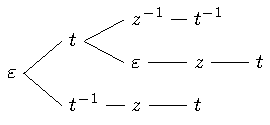
\includegraphics{figures/geodesicGenerating/treeRep}

	\caption{Tree representation of a geodesic equivalence class}
	\label{fig:tree1}
\end{figure}


Then, reading the nodes of the above tree from root to leaves, this tree represents the collection of words $tz^{-1}t^{-1}$, $tzt$, and $t^{-1}z t$.
Notice that each $\varepsilon$ is ignored when constructing words.

Given a tree of this form, the words can be extended a single letter in constant time.
For example, the words of the tree given earlier (in \cref{fig:tree1}) could be extended by the letter $z$ by adding a single edge to obtain the  tree in \cref{fig:tree2}, now rooted at $z$.

\begin{figure}[!ht]
	\centering

	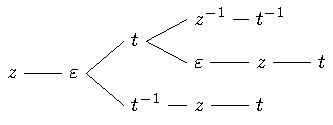
\includegraphics{figures/geodesicGenerating/treeRep2}

	\caption{The tree from \cref{fig:tree1}, extended by the letter $z$}
	\label{fig:tree2}
\end{figure}

Further, trees of this form can be combined (i.e.\ their words combined into one collection) in constant time, by adding two edges and a single node.
For example, consider the following union shown in \cref{fig:tree3}.

\begin{figure}[h!]
\begin{center}
	\begin{tabular}{m{3.5cm} m{1em} m{3.5cm} m{2em} m{4.5cm}}
		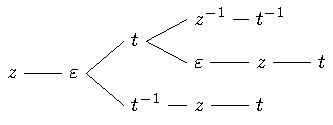
\includegraphics[width=3.5cm]{figures/geodesicGenerating/treeRep2}
		&
		\hfill
		$\bigcup$
		\hfill
		&
		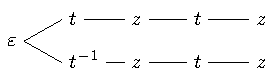
\includegraphics[width=3.5cm]{figures/geodesicGenerating/treeRep3}
		&
		\hfill
		$\Longrightarrow$
		\hfill
		&
		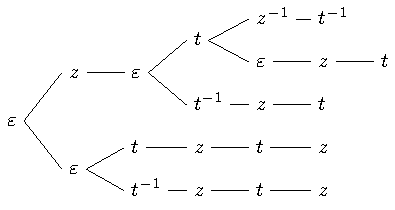
\includegraphics[width=4.5cm]{figures/geodesicGenerating/treeRep4Combined}
	\end{tabular}
\end{center}
\caption{Union of two rooted trees.}
	\label{fig:tree3}
\end{figure}


Thus, collections of words can be represented as tuples of the form $(w,B,T)$ where $w \in X^\ast$ is a representative of the collection, $B \subseteq X$ is the list of letters which begin words in the collection, and $T$ is a rooted tree as described earlier.
Using such tuples, it can be seen that collections of length $n-1$ geodesic can be extended to a collection of length $n$ words in constant time.
Thus, the list of length $n$ words can be produced in time $O(s(n-1))$, rather than $O(S(n-1))$.
Hence, it will be taken that $f(n) = 2 \cdot s(n-1)$ where $f(n)$ is as described at the beginning of this section, and $2 \cdot s(n-1)$ is an upper bound on the number of collections of extended words.

\begin{remark}
	It would also be possible to use tuples of the for $(w,B,\ell)$ where $\ell\in \mathbb{N}_+$ is the size (i.e.\ number of words) of the collection.
	This form does not contain enough information to recover the list full list of geodesics in each collection, however, it would contain enough compute the geodesic growth as the sum of all such $\ell$'s in the output.
	\thmendmark
\end{remark}

Notice that in the worst case, with respect to time complexity, all geodesics of length $n-1$ can be extended to length $n$ words as in \cref{rmk:genrated-next-geodesics}.
Thus, the variable $k$, which was used to denote the number of length $n$ input words, is bounded from above by $2 \cdot s(n-1)$.

Thus, the time-complexity of the full brute force algorithm is
\[
  O\left(
    \sum_{\ell = 1}^n \Big( 2 \cdot s(\ell-1) + (2 \cdot s(\ell-1))^2 \ell \log \ell \Big)
  \right)
  =
  O\left(
    \gamma(n-1)
    +
    \sum_{\ell=1}^n s(\ell-1)^2 \, \ell \log \ell
  \right)
\]
Then, considering that $s(\ell-1) \leq s(\ell-1)^2 \ell \log \ell$ and that $\sum_{\ell=1}^n s(\ell-1) = \gamma(\ell-1)\geq \gamma(\ell-1)$ it can be seen that this time complexity can be simplified to
\[
  O\left(
    \sum_{\ell=1}^n s(\ell-1)^2 \, \ell \log \ell
  \right)
\]
The time-complexity of the full sort-based algorithm is
\[
  O\left(
    \sum_{\ell = 1}^n \Big(
        2 \cdot s(\ell-1)
        +
        \big[2 \cdot s(\ell-1)\log (2 \cdot s(\ell-1)) + 2 \cdot s(\ell-1)\big] \, \ell \log \ell 
    \Big)
  \right)
\]
which can then be simplified to
\[
	O\left(
	\gamma(n-1)
	+
	\sum_{\ell = 1}^n
	\big[2 \cdot s(\ell-1)\log (2 \cdot s(\ell-1)) + 2 \cdot s(\ell-1)\big] \, \ell \log \ell
	\right)
\]
Then, simplified to
\[
O\left(
\gamma(n-1)
+
\sum_{\ell = 1}^n s(\ell-1) \log s(\ell-1) \, \ell \log \ell
\right)
\]
Then, considering that $\sum_{\ell = 1}^n s(\ell-1) \log s(\ell-1) \, \ell \log \ell$ grows faster, asymptotically, then $\gamma(n-1)$, it can be seen that this complexity becomes
\[
O\left(
\sum_{\ell = 1}^n s(\ell-1) \log s(\ell-1)  \, \ell \log \ell
\right)
\]
Hence, the complexity of the brute force and sorting based methods are
\begin{align*}
  O\left(
  \sum_{\ell=1}^n s(\ell-1)^2 \, \ell \log \ell
  \right)
  &&\text{and}&&
  O\left(
  \sum_{\ell = 1}^n s(\ell-1) \log s(\ell-1) \, \ell \log \ell
  \right)
\end{align*}
respectively.

Thus, it can be seen that the sorting-based method provides a better time complexity then the brute force method, particularly when considering that $s(n)$ is superpolynomial in complexity \cite{OnGrowth}.
To see this improvement, consider the following example.

\begin{example}
	For the moment suppose that $s(n) = e^{\sqrt{n}}$.
	Then, the respective complexities of the brute force and sort-based methods would be
	\begin{align*}
	O\left(
	\sum_{\ell=1}^n e^{2 \sqrt{\ell-1}} \, \ell \log \ell
	\right)
	&&\text{and}&&
	O\left(
	\sum_{\ell = 1}^n e^{\sqrt{\ell-1}} \sqrt{\ell-1} \, \ell \log \ell
	\right)
	\end{align*}
	Now, consider the following
	\[
	  \frac
	  {\displaystyle \sum_{\ell=1}^n e^{2 \sqrt{\ell-1}} \, \ell \log \ell}
	  {\displaystyle  \sum_{\ell = 1}^n e^{\sqrt{\ell-1}} \sqrt{\ell-1} \, \ell \log \ell}
	  \geq
	  \frac
	  {\displaystyle e^{2 \sqrt{n-1}} \, n \log n}
	  {\displaystyle n \cdot \left( e^{\sqrt{n-1}} \sqrt{n-1} \, n \log n \right) }
	  \geq
	  e^{\sqrt{n-1}} / n^2
	\]
	Thus, the worst-case sorting based method is (asymptotically) faster than the worst-case brute force method by, at least, a factor that is a multiple of $e^{\sqrt{n-1}}/n^2$, which is itself superpolynomial.
	
	Further, it is known from \cite{OnGrowth} that the complexity of $s(n)$ is higher than that of $e^{\sqrt{n}}$, and thus the difference in (worst-case) time complexity would be even more pronounced for Fabrykowski-Gupta.
\end{example}

\begin{remark}
	Both the brute force and sorting based methods have been implemented, by the author, in the programming language C.
	In less than two minutes, the sort-based method generated more data than the brute force method could in two weeks.
	Further, in less than ten hours the sort-based method was able to generate more data than the brute force method would be able to if it were given five centuries of time to run.
\end{remark}



\chapter{Results}

The goal of this chapter is to analyse data generated by the algorithm presented in \cref{chp:generating-geodesics}.

\section{Growth Functions}

This section will provide a comparison of the geodesic and regular growth functions of the Fabrykowski-Gupta group.
The corresponding raw data of this section is provided in \cref{tab:strict-growths}.
Firstly, the regular and geodesic growth functions, $\gamma(n)$ and $\Gamma(n)$, are plotted in \cref{fig:normalGrowth}.

\begin{figure}[!h]
	\centering
	
	\begin{subfigure}{0.48\linewidth}
		\centering
		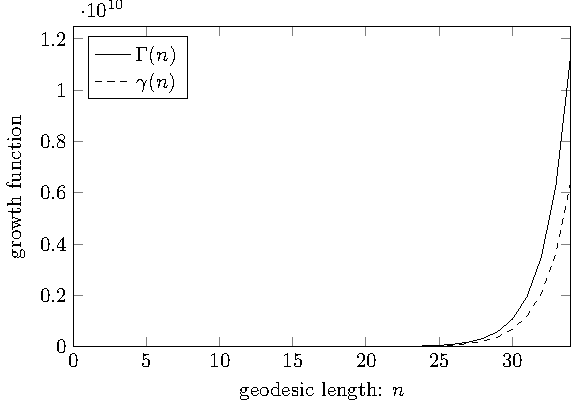
\includegraphics[width=\linewidth]
			{figures/results/normalGrowth/usual/normalGrowth}
		\caption{linear scale}
		\label{fig:normalGrowth:linear}
	\end{subfigure}
	\hfill
	\begin{subfigure}{0.48\linewidth}
		\centering
		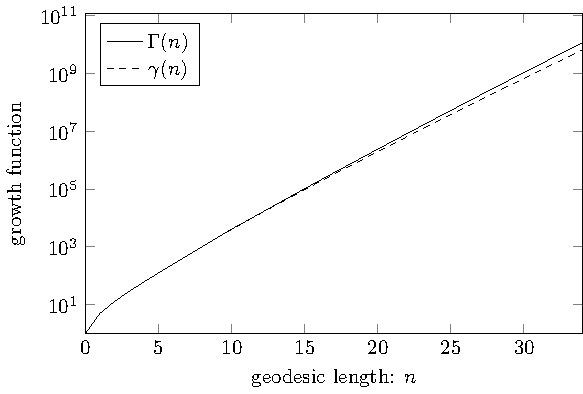
\includegraphics[width=\linewidth]
			{figures/results/normalGrowth/log/normalGrowthLog}
		\caption{logarithmic scale}
		\label{fig:normalGrowth:log}
	\end{subfigure}
	
	\caption{Comparison of the regular and geodesic growth functions}
	\label{fig:normalGrowth}
\end{figure}

Not much can be determined from \cref{fig:normalGrowth} as provided above.
Thus, to compare these two growth functions, the ratio $\Gamma(n)/\gamma(n)$ will instead be considered.
The ratio  $\Gamma(n)/\gamma(n)$ is of particular relevance as it can be shown that if this function is subexponential, then $\Gamma(n)$ would be of intermediate growth as would be desired.
An argument for this is given as follows.

We know  that $\Gamma(n)$ is superpolynomial since $\gamma \preccurlyeq \Gamma$ (see \cref{prop:growth-function-bounds}) and $\gamma(n)$ being superpolynomial \cite{OnGrowth}.
Also, it is known from \cite{OnGrowth} that $\gamma(n)$ is subexponential.
Hence, if $\Gamma(n)/\gamma(n)$ is subexponential, it would follow that the growth rate $\omega(\Gamma)$ could be computed as follows
\[
  \omega(\Gamma)
  =
  \lim_{n \to \infty}
  \frac{\log \Gamma(n)}{n}
  =
  \lim_{n \to \infty}
  \left(
  \frac{\log \gamma(n)}{n}
  +
  \frac{\log (\Gamma(n)/\gamma(n))}{n}
  \right)
  =
  \omega(\gamma)
  +
  \omega(\Gamma/\gamma)
\]
Then, since $\omega(\gamma) = 0$ and $\omega(\Gamma/\gamma) = 0$ by the definition of subexponential functions (see \cref{def:subexponential}), it follows that $\omega(\Gamma) = 0$; and thus $\Gamma(n)$ is subexponential.
Therefore, if $\Gamma(n)/\gamma(n)$ is subexponential, then it would follow that $\Gamma(n)$ is of intermediate growth.

Notice also that if $\Gamma(n)/\gamma(n)$ is exponential, then $\Gamma(n)$ would also be exponential.
This is clear as $\Gamma(n)/\gamma(n) \leq \Gamma(n)$ and thus $\Gamma/\gamma \preccurlyeq \Gamma$.
Thus, it can be seen that, if $\log(\Gamma(n)/\gamma(n))$ is linear, it would follow that $\Gamma(n)$ is exponential.
Hence, the function $\log(\Gamma(n)/\gamma(n))$ will also be considered.

Thus, consider the plots provided in \cref{fig:normalGrowthRatio}.

\begin{figure}[!h]
	\centering
	
	\begin{subfigure}{0.48\linewidth}
		\centering
		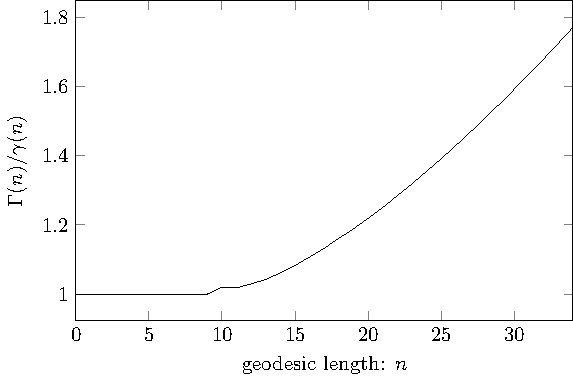
\includegraphics[width=\linewidth]
			{figures/results/normalGrowth/usual/normalGrowthRatio}
		\caption{Check for subexponential growth}
		\label{fig:normalGrowthRatio:linear}
	\end{subfigure}
	\hfill
	\begin{subfigure}{0.48\linewidth}
		\centering
		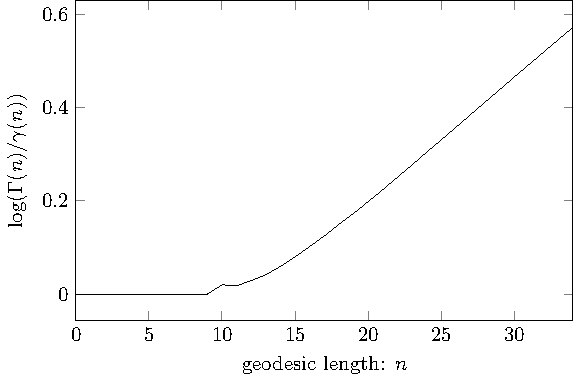
\includegraphics[width=\linewidth]
			{figures/results/normalGrowth/log/normalGrowthRatioLog}
		\caption{Check for exponential growth}
		\label{fig:normalGrowthRatio:log}
	\end{subfigure}
	
	\caption{Plots of $\Gamma(n)/\gamma(n)$ and $\log(\Gamma(n)/\gamma(n))$}
	\label{fig:normalGrowthRatio}
\end{figure}

The first derivatives (computed by the central difference) of these ratios are given in \cref{fig:normalGrowthRatioD1}.

\begin{figure}[!h]
	\centering
	
	\begin{subfigure}{0.48\linewidth}
		\centering
		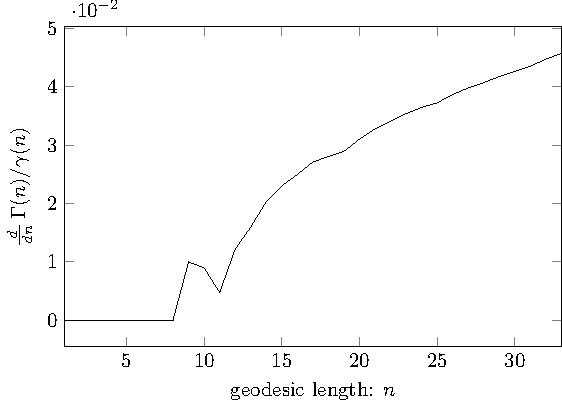
\includegraphics[width=\linewidth]
			{figures/results/normalGrowth/usual/normalGrowthRatioD1}
		\caption{First derivative of $\Gamma(n)/\gamma(n)$}
		\label{fig:normalGrowthRatio:linear:D1}
	\end{subfigure}
	\hfill
	\begin{subfigure}{0.48\linewidth}
		\centering
		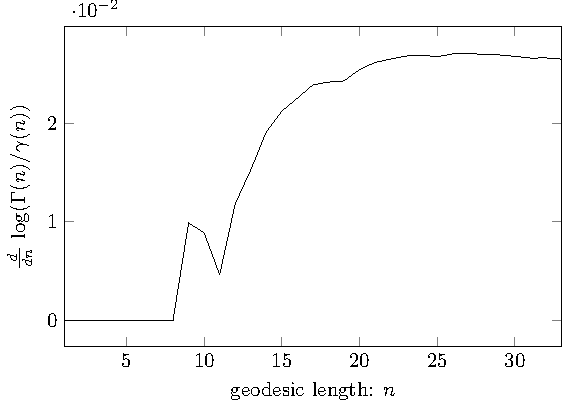
\includegraphics[width=\linewidth]
			{figures/results/normalGrowth/log/normalGrowthRatioLogD1}
		\caption{First derivative of $\log(\Gamma(n)/\gamma(n))$}
		\label{fig:normalGrowthRatio:log:D1}
	\end{subfigure}
	
	\caption{First derivatives of $\Gamma(n)/\gamma(n)$ and $\log(\Gamma(n)/\gamma(n))$}
	\label{fig:normalGrowthRatioD1}
\end{figure}

Further, the second and third derivatives (computed by the central difference) of $\Gamma(n)/\gamma(n)$ are given in \cref{fig:normalGrowthRatioD2D3}.

\begin{figure}[!h]
	\centering
	
	\begin{subfigure}{0.48\linewidth}
		\centering
		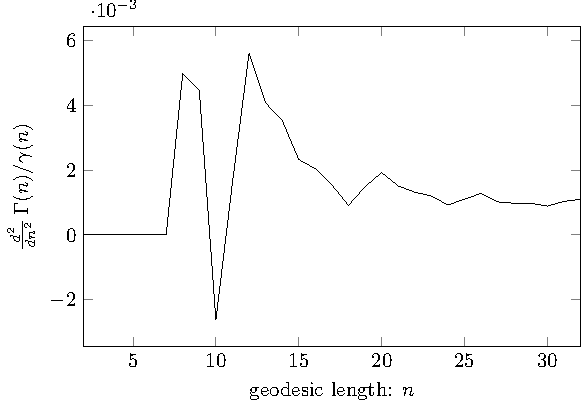
\includegraphics[width=\linewidth]
		{figures/results/normalGrowth/usual/normalGrowthRatioD2}
		\caption{Second derivative of $\Gamma(n)/\gamma(n)$}
		\label{fig:normalGrowthRatio:linear:D2}
	\end{subfigure}
	\hfill
	\begin{subfigure}{0.48\linewidth}
		\centering
		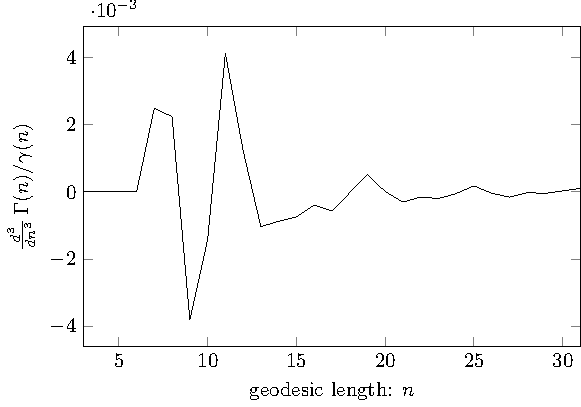
\includegraphics[width=\linewidth]
		{figures/results/normalGrowth/usual/normalGrowthRatioD3}
		\caption{Third derivative of $\Gamma(n)/\gamma(n)$}
		\label{fig:normalGrowthRatio:log:D3}
	\end{subfigure}
	
	\caption{Higher derivatives of $\Gamma(n)/\gamma(n)$}
	\label{fig:normalGrowthRatioD2D3}
\end{figure}

\newpage
\section{Geodesic Equivalence Class Size}

Similar to the previous section, for $\Gamma(n)$ to be subexponential and thus intermediate, it would be sufficient to show that the size of the largest geodesic equivalence class is subexponential with respect to the geodesic length $n$; and further, if such a function is exponential, the so is $\Gamma(n)$.
Thus, the size of the largest equivalence classes is given in \cref{fig:maximumEquivClassSize}.
The corresponding raw data of this section is given in \cref{tab:class-sizes}.

\begin{figure}[!h]
	\centering
	
	\begin{subfigure}{0.48\linewidth}
		\centering
		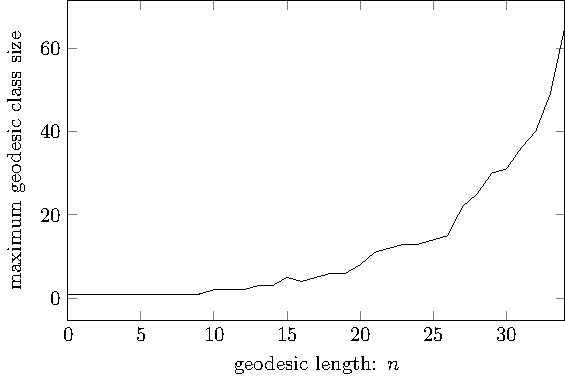
\includegraphics[width=\linewidth]
		{figures/results/maxClassSize/usual/maxClassSize}
		\caption{linear scale}
		\label{fig:maximumEquivClassSize:linear}
	\end{subfigure}
	\hfill
	\begin{subfigure}{0.48\linewidth}
		\centering
		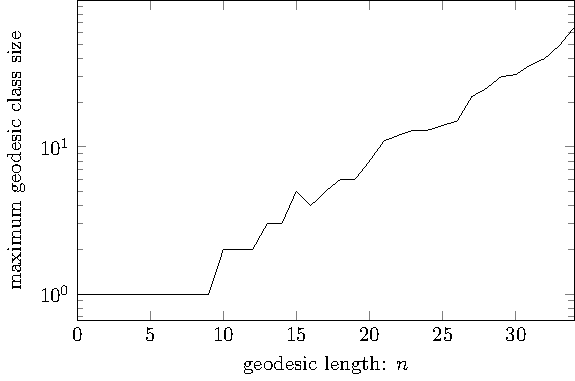
\includegraphics[width=\linewidth]
		{figures/results/maxClassSize/log/maxClassSizeLog}
		\caption{logatithmic scale}
		\label{fig:maximumEquivClassSize:log}
	\end{subfigure}
	
	\caption{The size of the largest equivalence classes}
	\label{fig:maximumEquivClassSize}
\end{figure}

\section{Remarks and Conjecture}

After generating the geodesics described in this section, graphs similar to the one on the front cover of this thesis were generated.
The graph on the cover represents a particular geodesic equivalence class of length 24 geodesics where the first node corresponds the group identity and the last node corresponds the group element represented by the geodesics.
Thus, such graphs can be understood to be sub-graphs of the Cayley graph of the Fabrykowski-Gupta group.

The idea behind generating graphs such as the one on the front cover was to see if any patterns presented themselves.
For example, if any exponential growth sub-families could be seen from such graphs.
The other patterns of this form have not been included in this thesis due to the large number of such graphs; there are $2311$ distinct graphs, of this form, of length 23 geodesics alone.

Considering the figures from the previous two sections, the author arrives at the following conjecture.

\begin{conjecture}
	The function $\Gamma(n)/\gamma(n)$ either grows slower than quadratic or is exponential of a small growth rate; thus either, $\Gamma \preccurlyeq n^2 \gamma$ or $\Gamma(n)$ is exponential of a small growth rate.
\end{conjecture}



\clearpage
\phantomsection

\addcontentsline{toc}{chapter}{Bibliography}
\printbibliography

\appendix

\chapter{Pseudocode}
\label{apx:modified-mergesort}

\section{Final Merge Algorithm}
\label{apx:final-merge}

\begin{algorithm}[h!]
	
	\Fn(){\MERGEFINAL{$\mathcal{S}, \mathcal{T}$}}{
		\KwData{sorted lists $\mathcal{S}$ of length $n$ geodesics and $\mathcal{T}$ of length $n+1$ extended words}
		\KwResult{returns the length $n+1$ geodesics}
		
		\BlankLine
		
		\tcp{Initialise the output list to empty}
		$\mathcal{L}$ $\gets$ $()$\;
		
		\BlankLine
		
		\tcp{$i$ and $j$ index the lists $\mathcal{S}$ and $\mathcal{T}$ respectively}
		$i$ $\gets$ $0$\;
		$j$ $\gets$ $0$\;
		
		\BlankLine
		
		\tcp{$n$ and $m$ are the sizes of the lists $\mathcal{S}$ and $\mathcal{T}$ respetively}
		$n$ $\gets$ $\left\vert S \right\vert$\;
		$m$ $\gets$ $\left\vert T \right\vert$\;
		
		\BlankLine
		
		\tcp{The following merges the lists until the end of one is reached}
		
		\BlankLine
		
		\While{$i \leq n$ and $j \leq m$}{
			
			cmp $\gets$ \COMP($\textrm{rep}(\mathcal{S}_{i})$, $\textrm{rep}(\mathcal{T}_{j})$)\tcc*{compare the equivalence classes}
			
			\BlankLine
			
			\uIf{$\text{cmp} = 0$}{
				
				\tcp{$\mathcal{T}_j$ is not a geodesic $n+1$}
				
				$i$ $\gets$ $i+1$\;
				$j$ $\gets$ $j+1$\;
			}
			\uElseIf{$\text{cmp} < 0$}{
				\tcp{$\mathcal{S}_i < \mathcal{T}_j$}
				
				$i$ $\gets$ $i+1$\;
			}
			\Else{
				append $\mathcal{T}_j$ to $\mathcal{L}$\tcc*{$\mathcal{T}_i < \mathcal{S}_j$ and thus $\mathcal{T}_i$ should be added next}
				
				$j$ $\gets$ $j+1$\;
			}
		}
		
		\BlankLine
		
		\tcp{The following adds any remaining elements $\mathcal{T}$ to $\mathcal{L}$}
		
		\If{$j < m$}{
			append $\mathcal{S}_j, \mathcal{S}_{j+1}, \ldots, \mathcal{S}_{m}$ to $\mathcal{L}$\;
		}
		
		\BlankLine
		
		\tcp{$\mathcal{L}$ will now contain the list of length $n+1$ geodesics}
		
		\BlankLine
		
		\Return{$\mathcal{L}$}\;
		
	}
	
	\caption{Merges a list of length $n$ geodesics with length $n+1$ words}
	\label{alg:mergesort:finalmerge}
\end{algorithm}

\newpage
\section{Merge Algorithm}
\label{apx:modified-mergesort:merge}

\begin{algorithm}[h!]
	
	\Fn(){\MERGE{$\mathcal{S}, \mathcal{T}$}}{
		\KwData{two sorted lists, $\mathcal{S}$ and $\mathcal{T}$, of collections of length $n+1$ words to merge}
		\KwResult{returns the merged list}
		
		\BlankLine
		
		\tcp{Initialise the output list to empty}
		$\mathcal{L}$ $\gets$ $()$\;
		
		\BlankLine
		
		\tcp{$i$ and $j$ index the lists $\mathcal{S}$ and $\mathcal{T}$ respectively}
		$i$ $\gets$ $0$\;
		$j$ $\gets$ $0$\;
		
		\BlankLine
		
		\tcp{$n$ and $m$ are the sizes of the lists $\mathcal{S}$ and $\mathcal{T}$ respetively}
		$n$ $\gets$ $\left\vert S \right\vert$\;
		$m$ $\gets$ $\left\vert T \right\vert$\;
		
		\BlankLine
		
		\tcp{The following merges the lists until the end of one is reached}
		
		\BlankLine
		
		\While{$i \leq n$ and $j \leq m$}{
			
			\BlankLine
			
			cmp $\gets$ \COMP($\textrm{rep}(\mathcal{S}_{i})$, $\textrm{rep}(\mathcal{T}_{j})$)\tcc*{compare the equivalence classes}
			
			\BlankLine
			
			\uIf{$\text{cmp} = 0$}{
				
				append $\mathcal{S}_{i} \cup \mathcal{T}_{j}$ to $\mathcal{L}$\tcc*{The collections should be combined}
				
				\BlankLine
				
				$i$ $\gets$ $i+1$\;
				$j$ $\gets$ $j+1$\;
			}
			\uElseIf{$\text{cmp} < 0$}{
				append $\mathcal{S}_i$ to $\mathcal{L}$\tcc*{$\mathcal{S}_i < \mathcal{T}_j$ and thus $\mathcal{S}_i$ should be added next}
				
				$i$ $\gets$ $i+1$\;
			}
			\Else{
				append $\mathcal{T}_j$ to $\mathcal{L}$\tcc*{$\mathcal{T}_i < \mathcal{S}_j$ and thus $\mathcal{T}_i$ should be added next}
				
				$j$ $\gets$ $j+1$\;
			}
		}
		
		\BlankLine
		
		\tcp{The following adds any remaining elements of $\mathcal{S}$ and $\mathcal{T}$ to $\mathcal{L}$}
		
		\BlankLine
		
		\If{$i < n$}{
			append $\mathcal{S}_i, \mathcal{S}_{i+1}, \ldots, \mathcal{S}_{n}$ to $\mathcal{L}$\;
		}
		
		\BlankLine
		
		\If{$j < m$}{
			append $\mathcal{S}_j, \mathcal{S}_{j+1}, \ldots, \mathcal{S}_{m}$ to $\mathcal{L}$\;
		}
		
		\BlankLine
		
		\tcp{$\mathcal{L}$ will now contain the merged lists}
		
		\BlankLine
		
		\Return{$\mathcal{L}$}\;
		
	}
	
	\caption{Merges two lists of length $n+1$ extended words}
	\label{alg:mergesort:merge}
\end{algorithm}

\newpage
\section{Main Sort Algorithm}
\label{apx:modified-mergesort:sort}

\begin{algorithm}[h!]
	
	\Fn(){\SORT{$\mathcal{L}$}}{
		\KwData{an unsorted list of length $n+1$ extended words $\mathcal{L}$}
		\KwResult{returns a list of sorted words}
		
		\BlankLine
		
		\tcp{If $\mathcal{L}$ contains one or zero collections, then it is already sorted}
		
		\If{$\left\vert \mathcal{L} \right\vert \leq 1$}{
			\Return $\mathcal{L}$
		}
		
		\BlankLine
		
		\tcp{If $\mathcal{L}$ is size $2$ then it should be sorted and returned}
		
		\If{$\left\vert \mathcal{L} \right\vert = 2$} {
			cmp $\gets$ \COMP($\textrm{rep}(\mathcal{L}_1)$, $\textrm{rep}(\mathcal{L}_2)$)\tcc*{compare the elements of the list}
			
			\BlankLine
			
			\uIf{$\text{cmp} = 0$}{
				
				\Return{$(\mathcal{L}_1 \cup \mathcal{L}_2)$}\tcc*{the collections should be combined}
				
			}
			\uElseIf{$\text{cmp} < 0$}{
				\Return{$\mathcal{L}$}\tcc*{the list is already in the correct order}
			}
			\Else{
				\Return{$(\mathcal{L}_2, \mathcal{L}_1)$}\tcc*{the list was not sorted}
			}
			
		}
		
		\BlankLine
		
		\tcp{$n$ is the length of the the list and $m$ is its midpoint}
		
		$n$ $\gets$ $\left\vert \mathcal{L} \right\vert$\;
		$m$ $\gets$ $\left\lceil n / 2 \right\rceil$\;
		
		\BlankLine
		
		\tcp{Seperate the list into two parts based on the midpoint}
		
		left  $\gets$ $(\mathcal{L}_1, \mathcal{L}_2, \ldots, \mathcal{L}_{m})$\;
		right $\gets$ $(\mathcal{L}_{m+1},\mathcal{L}_{m+2},\ldots,\mathcal{L}_{n})$\;
		
		\BlankLine
		
		\tcp{Sort the two parts of the list}
		
		$\mathcal{S}_{\text{left}}$  $\gets$ \SORT(left)\;
		$\mathcal{S}_{\text{right}}$ $\gets$ \SORT(right)\;
		
		\BlankLine
		
		\tcp{Merge the sorted lists and return the result}
		
		\Return{\MERGE($\mathcal{S}_\text{left}$, $\mathcal{S}_\text{right}$)}\;
	}
	
	\caption{Sorts a list of geodesics}
	\label{alg:mergesort:sort}
\end{algorithm}


\chapter{Generated Data}
\label{apx:generated-data}

\begin{table}[!ht]
	\centering
	\begin{tabular}{
			| S[table-format=2.0]
			| S[table-format=10.0]
			| S[table-format=10.0]
			|
		}
		\hline
		\multicolumn{1}{|c|}{Word Length: $n$} &
		\multicolumn{1}{c|}{Strict Growth: $s(n)$} &
		\multicolumn{1}{c|}{Strict Geodesic Growth: $S(n)$}
		\\
		\hline\hline
		0 & 1 & 1 \\\hline
		1 & 4 & 4 \\\hline
		2 & 8 & 8 \\\hline
		3 & 16 & 16 \\\hline
		4 & 32 & 32 \\\hline
		5 & 64 & 64 \\\hline
		6 & 128 & 128 \\\hline
		7 & 256 & 256 \\\hline
		8 & 512 & 512 \\\hline
		9 & 1024 & 1024 \\\hline
		10 & 1968 & 2048 \\\hline
		11 & 3608 & 3664 \\\hline
		12 & 6816 & 7104 \\\hline
		13 & 12704 & 13424 \\\hline
		14 & 23696 & 25664 \\\hline
		15 & 43720 & 48432 \\\hline
		16 & 80224 & 91136 \\\hline
		17 & 146432 & 170304 \\\hline
		18 & 266688 & 318944 \\\hline
		19 & 484464 & 591984 \\\hline
		20 & 878800 & 1104032 \\\hline
		21 & 1589376 & 2049584 \\\hline
		22 & 2862976 & 3797952 \\\hline
		23 & 5145456 & 7004976 \\\hline
		24 & 9226328 & 12928032 \\\hline
		25 & 16495488 & 23712040 \\\hline
		26 & 29422368 & 43491840 \\\hline
		27 & 52346136 & 79512504 \\\hline
		28 & 92872704 & 144997904 \\\hline
		29 & 164374672 & 263539944 \\\hline
		30 & 290176048 & 478231104 \\\hline
		31 & 511135408 & 864602376 \\\hline
		32 & 897966344 & 1560704000 \\\hline
		33 & 1573794776 & 2808866784 \\\hline
		34 & 2751740432 & 5043285984 \\\hline
	\end{tabular}
	\caption{Results of the strict growth functions}
	\label{tab:strict-growths}
\end{table}

\begin{table}[!ht]
	\centering
	\begin{tabular}{
			| S[table-format=2.0]
			| S[table-format=2.0]
			|
		}
		\hline
		\multicolumn{1}{|c|}{Word Length: $n$} &
		\multicolumn{1}{c|}{Largest Geodesic Equivalence Class Size}
		\\
		\hline\hline
		0 & 1 \\\hline
		1 & 1 \\\hline
		2 & 1 \\\hline
		3 & 1 \\\hline
		4 & 1 \\\hline
		5 & 1 \\\hline
		6 & 1 \\\hline
		7 & 1 \\\hline
		8 & 1 \\\hline
		9 & 1 \\\hline
		10 & 2 \\\hline
		11 & 2 \\\hline
		12 & 2 \\\hline
		13 & 3 \\\hline
		14 & 3 \\\hline
		15 & 5 \\\hline
		16 & 4 \\\hline
		17 & 5 \\\hline
		18 & 6 \\\hline
		19 & 6 \\\hline
		20 & 8 \\\hline
		21 & 11 \\\hline
		22 & 12 \\\hline
		23 & 13 \\\hline
		24 & 13 \\\hline
		25 & 14 \\\hline
		26 & 15 \\\hline
		27 & 22 \\\hline
		28 & 25 \\\hline
		29 & 30 \\\hline
		30 & 31 \\\hline
		31 & 36 \\\hline
		32 & 40 \\\hline
		33 & 49 \\\hline
		34 & 65 \\\hline
	\end{tabular}
	\caption{Largest geodesic equivalence class sizes}
	\label{tab:class-sizes}
\end{table}


\end{document}